\documentclass{EESD}
% To change the slides size go to EESD.cls file and edit the preamble as explained.

% Show notes on second screen
\setbeameroption{show notes on second screen=right}

% Important packages to be called
\usepackage{subcaption} % for adding sub-figures
\usepackage{graphicx}
\usepackage{tikz} % for cool graphics and drawings
\usepackage{multimedia} % for embedded multimedia files
\usepackage[final]{pdfpages} % include pdf figures

\usepackage[absolute,overlay]{textpos} % To place the figures by coordinates (x,y) - Beamer doesn't support floats XD
\usepackage{multicol} % To adjust items and stuff automatically in a number of a pre-specified columns
\graphicspath{{Figures/}}
\usepackage[utf8]{inputenc}
\usepackage{amsmath}
\usepackage{amsfonts}
\usepackage{amssymb}
\usepackage{lipsum} % Just a dummy text generator
\usepackage{hyperref}
% fonts packages
\usepackage{ragged2e} % Justified typesetting

% For References Only
\usepackage[style=authortitle,backend=bibtex]{biblatex}
\addbibresource{references.bib} % Call the references database
\AtBeginBibliography{\tiny} % Specify font size (Size matters)
\renewcommand{\footnotesize}{\tiny}

% For adding code blocks
\usepackage{listings}
\lstset
{
    language=[LaTeX]TeX,
    breaklines=true,
    basicstyle=\tt\scriptsize,
    keywordstyle=\color{blue},
    identifierstyle=\color{magenta},
    commentstyle=\color{red},
    rulecolor=\color{black},
    numbers=left,
    numberstyle=\tiny\color{black},
    % framexleftmargin=15pt,
    frame = single,
}

% ---- Add your Meta-data to the PDF (Copyrights Kinda!) ----
\hypersetup{
  pdfinfo={
    Title={Inter-seasonal Performance of Gaussian
Process-based Model Predictive Control of
Buildings},
    Author={Radu C. Martin},
    Subject={EPFL - IGM - LA3 Lab},
    Keywords={Model Predictive Control, Gaussian Process, Sparse Variational
    Gaussian Process}
  }
}

\author{Radu C. Martin}
\title[Inter-seasonal Performance of GP-based MPC of Buildings]
    {Inter-seasonal Performance of Gaussian Process-based Model Predictive Control of Buildings}

\institute[IGM]{{\'Ecole Polytechnique F\'ed\'erale de Lausanne
(EPFL)}{\newline\newline Institute of Mechanical Engineering (IGM)}}
\subject{Master Thesis Defense}
\date{\today}


\begin{document}
    {
\coverpage{
\titlepage{~}
% To add additional text to the title components 
{\newline \small \textit{Supervisor}: Prof. Colin Jones \quad \textit{Assistant}: Manuel Koch \quad
\textit{Expert}: Bratislav Svetozarevic}
\note[item]{Introduction, welcome}
\note[item]{Present yourself and the thesis subject}
\note[item]{Analysis of GP models performance for longer lasting simulations, in
this case a full year}
\note[item]{Discussion of the shortcomngs of classical GP approaches for these
longer experiments and possible solutions}
}
}

\setbeamertemplate{logo}{} % To override the logo from the other slides and delete it completely


% Use smart division for the TOC
\begin{frame}{Outlines}
\begin{multicols}{2}
\tableofcontents
\end{multicols}
\note[item]{The main work consists of two parts: the CARNOT building model serving as
a plant for the simulation, and the definition and analysis of different GP/SVGP
based control schemes}
\note[item]{Starting with a short introduction where the motivation for these new
approaches is presented, followed by the basic ideas of GP models}
\end{frame}

% -----------------------Introduction
\section{Introduction}

\breakingframe{
\begin{textblock*}{3cm}[0.5,0.5](0.5\textwidth,  0.5\textheight)
\Huge\textbf{\textcolor{black}{Introduction}}
\end{textblock*}
}


\subsection{Residential buildings}

\begin{frame}[t]{Residential buildings energy usage}
    \begin{itemize}
        \item Residential buildings represent more than 25\% of total energy
            consumed in the EU \vspace{10pt} \pause
        \item Average of 200-300 kWh/year/m$^{2}$ \vspace{10pt} \pause
        \item Around 68\% of energy used for heating \vspace{10pt}
    \end{itemize}

    \note[item]{Residential buildings are a significant part of total energy
    consumption in the EU}
    \note[item]{Most of that energy is used for heating and ventilation of
    buildings}
    \note[item]{Additionally, there are increasing energy efficiency demands on
    new and existing buildings}
    \note[item]{Further improvements can be made by including already existing
    buildings into "smart grids"}
\end{frame}

\begin{frame}
    \frametitle{Limited information available}
    \begin{block}{Existing infrastructure}
    Most existing buildings already have in place Heating and Ventilation
    Systems:\pause
    \vspace{10pt}
    \begin{itemize}
        \item Limits the amount of available information \vspace{10pt} \pause
        \item Restricts the actionable signals to those provided by the existing
            HVAC \vspace{10pt}
    \end{itemize}
    \end{block}
    \pause
    \begin{block}{Weather forecast}
    Predictions of future disturbance values for the MPC also impose
    restrictions on usable data.
    \end{block}
    \note[item]{Polydome only has two temperature measurements}
    \note[item]{Existing data lacks information on air humidity}
    \note[item]{Existing data lacks information on occupancy\vspace{10pt}}
    \note[item]{The only input for the Polydome's HVAC is the setpoint
    temperature, thus only indirectly controlling the heat input\vspace{10pt}}
    \note[item]{Weather predictions are restricted to outside temperature and
    GHI}
    \note[item]{This makes the use of other disturbances, such as humidity,
    wind speed and direction, DNI, DHI inaccessible}
\end{frame}

\subsection{Black box models}

\begin{frame}
    \frametitle{Black-box models}
    Data-driven models provide several practical benefits over first-principle
    models:
    \vspace{10pt}
    \begin{itemize}
        \item Foregoes complex and potentially expensive physical modelling \vspace{10pt} \pause
        \item Same data-driven model structure could be applied to other
            situations with less effort \vspace{10pt} \pause
        \item Unknown/complex plant elements, such as HVAC behaviour, unknown
            material properties , occupancy levels are much easier to include\vspace{10pt} \pause
    \end{itemize}
    \note[item]{In this context it would be very useful to be able to use
    data-driven models as they provide several benetifs over white-box
approaches:}
    \note[item]{They forego the complex physical modelling step}
    \note[item]{Applying a control scheme using a white-box model requires a
    complete identification step, whereas for data-driven models only the
hyperparameters have to be tuned}
    \note[item]{For buildings where not all information is readily available,
    white-box models can prove infeasible (eg. The Polydome building :D)}
\end{frame}


% ----------------------- Gaussian Process Models
\section{Gaussian Process Models}

\breakingframe{
\begin{textblock*}{13cm}[0.5,0.5](0.7\textwidth,  0.5\textheight)
\Huge\textbf{\textcolor{black}{Gaussian Process Models}}
\end{textblock*}
}

\subsection{Conventional Gaussian Processes}

\begin{frame}
    \begin{block}{Definition}
        A Gaussian Process is a collection of random variables, any finite
        number of which have a joint Gaussian distribution.
    \end{block}
    \begin{block}{Mathematical formulation}
        \begin{equation*}
                \begin{aligned}
                    m(\mathbf{x}) &= \mathbb{E}[f(\mathbf{x})] \\
                    k(\mathbf{x}, \mathbf{x'}) &= \mathbb{E}[f(\mathbf{x} -
                    m(\mathbf{x}))(f(\mathbf{x'}) - m(\mathbf{x'}))]
                \end{aligned}
        \end{equation*}
    \end{block}
    \note[item]{The formal definition of a Gaussian Process states that it is a
    collection of random variables, any finite number of which have a joint
    Gaussian distribution.}
    \note[item]{Another useful way of thinking of GPs is as a probability distribution, but over functions rather than variables. This is a really useful thing, as often in machine learning what we are trying to do is some form of function approximation. A GP allows us to derive posterior distributions over functions by simply observing variables.}
\end{frame}

\begin{frame}
    \frametitle{Benefits}
    \begin{itemize}
        \item Provide a complete Gaussian distribution for a predicted value
            \vspace{10pt} \pause
        \item Capture complex system behaviour with less data \vspace{10pt}
            \pause
        \item Include prior beliefs and impose desired model behaviour
            \vspace{10pt} \pause
            \begin{itemize}
                \item Different kernels can lead to linear, periodic, smooth
                    functions \vspace{10pt}
                \item Combinations of multiple kernel functions can impose
                    arbitrary behaviour \vspace{10pt}
                \item Ability to impose a prior distribution on hyperparameters
                    before training \vspace{10pt}
            \end{itemize}
    \end{itemize}
\end{frame}

\begin{frame}
    \frametitle{Shortcomings}

    \begin{block}{Predicting new values}
        \begin{equation*}
                \begin{aligned}
                    \mathbf{f_*} = \mathbb{E}\left(f_*|X, \mathbf{y}, X_*\right) &=
                    K_*\left(K + \sigma_n^2I\right)^{-1}\mathbf{y} \\
                    cov(\mathbf{f_*}) &= K_{**} - K_*\left(K +\sigma_n^2I\right)^{-1}K_*^T \\
                \end{aligned}
        \end{equation*}
    \end{block}

    \begin{block}{Maximum likelihood}
        \begin{equation*}
                \log(p(y)) = - \frac{1}{2}\log{\left(
                                \det{\left(
                                        K + \sigma_n^2I
                                \right)}
                            \right)}
                - \frac{1}{2}y^T\left(
                                    K + \sigma_n^2I
                                \right)^{-1}y
                - \frac{n}{2}\log{\left(2\pi\right)}
        \end{equation*}
    \end{block}

    \pause
    \begin{itemize}
        \item $\mathcal{O}(n^3)$ time for evaluation
        \item $\mathcal{O}(n^4)$ time for training
        \item $\mathcal{O}(n^2)$ space for finished model
    \end{itemize}
    \note[item]{Both training and evaluation require inversion of the covariance
    matrix}
    \note[item]{Impractical for embedded computers (slow, little memory)}
    \note[item]{Impractical for systems with faster dynamics}
    \note[item]{Impractical for complex systems where more data is needed to
    capture model behaviour}
\end{frame}

\subsection{Sparse and Variationsl Gaussian Processes}

\begin{frame}
    \frametitle{Sparse and Variational Gaussian Processes}
    Extension of classical Gaussian Processes for use on larger scale datasets
    \pause
    \begin{block}{Sparse}
        Approximating the full training dataset with a smaller number of points:
        \\
        \quad \textit{Inducing random variables} $f(X_s)$ at \textit{inducing
        locations} $X_s$
    \end{block}
    \pause
    \begin{block}{Variational}
    Variational inference uses the \textit{variational
    distribution} $q(f, f_s)$ to approximate the true posterior $p(f, f_s|y)$ \\
    This approximation leads to the \textit{Evidence Lower Bound} (ELBO), used
    for parameter training
    \end{block}
    \note[item]{Extension of classical GP meant to aleviate its shortcomings}
    \note[item]{Inducing random variables are a new set of learnable parameters
    trained in such a way to generate the original dataset as close as possible.
They are trained at the same time as the model, and when the original inputs are
evaluated on this new model the outputs should as close as possible ressemble
the original dataset outputs}
    \note[item]{With variational inference we approximate the true posterior
    distribution of the Gaussian process with the variational distribution}
    \note[item]{ELBO approximation allows training of the model on subsets
    (minibatches) of the original data}
\end{frame}


% ----------------------- CARNOT Model
\section{CARNOT Model}

\breakingframe{
\begin{textblock*}{13cm}[0.5,0.5](0.7\textwidth,  0.5\textheight)
\Huge\textbf{\textcolor{black}{CARNOT Building Model}}
\end{textblock*}
}

\begin{frame}
    \frametitle{Motivation}
    \begin{block}{Using CARNOT model as plant}
        \vspace{10pt}
        \begin{itemize}
            \item Much faster than real-time simulations \vspace{10pt}
                % allow for easier long-term performance evaluations
            \item Reproducible weather/ disturbances \vspace{10pt}
                % allows a much more direct comparison of different model
                % performances
        \end{itemize}
    \end{block}

    \begin{block}{Using the real Polydome building as basis}
        Experimental data already available
        \vspace{10pt}
        \begin{itemize}
            \item  Good baseline for comparing the CARNOT model to a real
                building \vspace{10pt}
            \item  Path to easier implementation of same control scheme on the
                real Polydome \vspace{10pt}
        \end{itemize}
    \end{block}
\end{frame}

\subsection{The Polydome building}

\begin{frame}
    \frametitle{Geometrical parameters}
    % TODO: [CARNOT] Geometrical parameters of the Polydome
    \begin{columns}
        \begin{column}{0.3\textwidth}
            \centering
            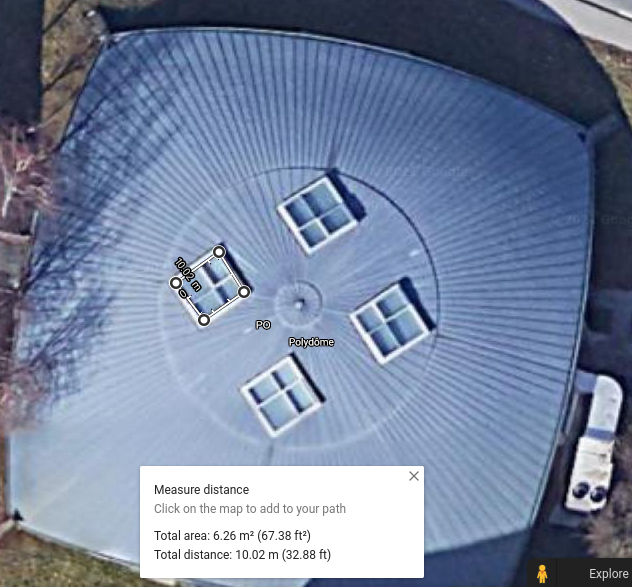
\includegraphics[height=\textwidth]{Images/google_maps_polydome_skylights.png}
        \end{column}
        \begin{column}{0.7\textwidth}
            \centering
            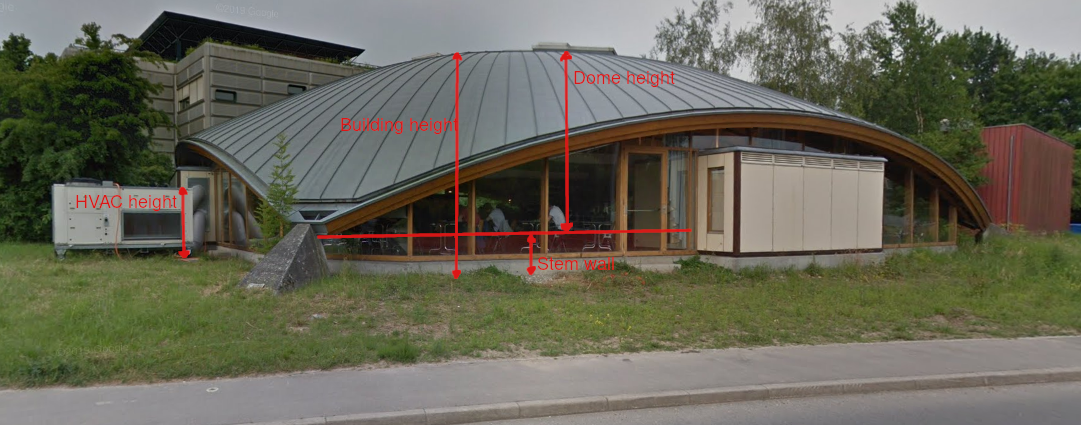
\includegraphics[height=0.45\textwidth]{Images/polydome_streetview_annotated.png}
        \end{column}
    \end{columns}

    \note[item]{Base geometrical dimensions from an architectural journal
    article on the Polydome construction:
        \begin{itemize}
            \item Spherical dome shape with a mostly square base of size 25m $\times$
                25m
            \item Total building height of around 7 meters
        \end{itemize}
    }
    \note[item]{Confirmation of surface from google maps, as well as
    approximation of skylights shape\vspace{10pt}}
    \note[item]{Overall building approximated with a spherical dome on top of a
    cylindrical stem wall}
    \note[item]{Google Street View capture of the Polydome building. An object
    of known dimensions is used (HVAC) as a scale and the necessary dimensions
    are measured with the Measure Tool in GIMP
        \begin{itemize}
            \item Steam wall size
            \item Dome height
            \item Total building height (used for validation of results)
        \end{itemize}
    }
\end{frame}

\begin{frame}
    \begin{block}{Materials used in the Polydome}
    \vspace{10pt}
    \begin{itemize}
        \item Walls are replaced with large, top to bottom windows \vspace{10pt}
        \item Roof made of insulation, enclosed by wood on each side
            \vspace{10pt}
        \item Floor consists of wood, insulation, concrete \vspace{10pt}
    \end{itemize}
    \end{block}
    \pause
    \begin{block}{Furniture}
        Approximated to a wall made out of \textit{equivalent indoor content
        material} with material properties and geometrical dimension to emulate
        real furniture.
    \end{block}

    \note[item]{Materials used in Polydome}
    \note[item]{Furniture is an important factor in building thermal inertia. In
    this case the existing furniture has been approximated to a wall with
geometrical and material properties to best emulate the real furniture}
    \note[item]{Furniture material parameters come from a study on the influence
    of furniture content on building thermal inertia and are representative of
an office environment}
\end{frame}

\subsection{CARNOT Model overview}

\begin{frame}
    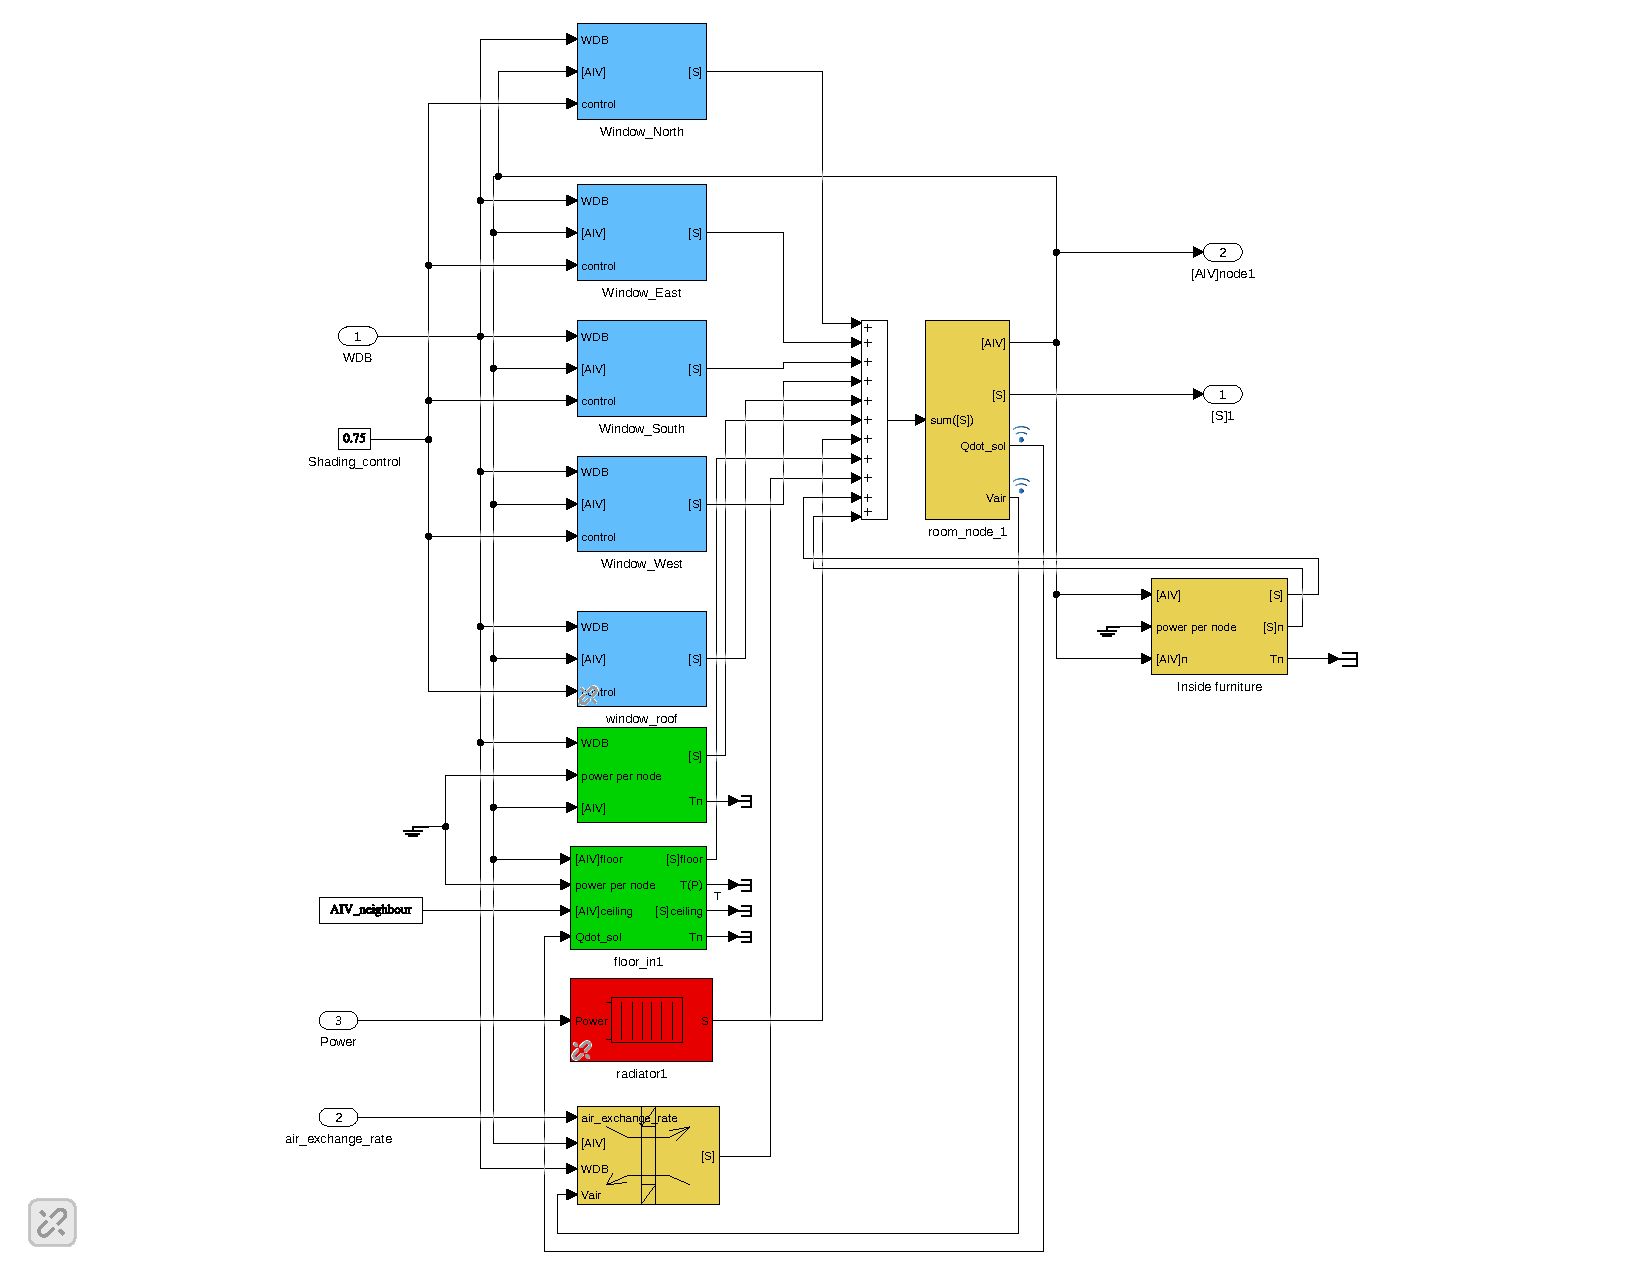
\includegraphics[height=\textheight]{Images/polydome_room_model.pdf}
    \note[item]{Four of the five window nodes represent the building walls}
    \note[item]{An additional window accounts for the skyboxes on the building
    roof\vspace{10pt}}
    \note[item]{Roof and floor made out of the appropriate materials}
    \note[item]{A wall with the purpose of approximating the furniture content
    of the building\vspace{10pt}}
    \note[item]{The heat radiator assumed to be ideal}
\end{frame}


% ----------------------- MPC Problem
\section{The MPC Problem}

\breakingframe{
\begin{textblock*}{13cm}[0.5,0.5](0.75\textwidth,  0.5\textheight)
\Huge\textbf{\textcolor{black}{The MPC Problem}}
\end{textblock*}
}

\begin{frame}
    \begin{block}{The Optimisation Problem}
    \begin{equation*}
            \begin{aligned}
                & \text{minimize}
                & & \sum_{i=0}^{N-1} (\bar{y}_{t+i} - y_{ref, t})^2 \\
                & \text{subject to}
                & & \bar{y}_{t+i} = K_*K^{-1}\mathbf{x}_{t+i-1} \\
                &&& \mathbf{x}_{t+i-1} = \left[\mathbf{w}_{t+i-1},\quad
                \mathbf{u}_{t+i-1},\quad \mathbf{y}_{t+i-1}\right]^T \\
                \label{eq:components}
                &&& u_{t+i} \in \mathcal{U}
            \end{aligned}
    \end{equation*}
    \end{block}
    \note[item]{The Problem of tracking a reference temperature subject to:
        \begin{itemize}
            \item Model constraints
            \item Future disturbance inputs
            \item Allowed input range (HVAC heating/cooling capacity)
        \end{itemize}
    }
    \note[item]{Choosing this specific optimisation problem allows easier
    comparison of different model performances, since they are directly
following the reference temperature}
\end{frame}

\begin{frame}
    \frametitle{Reference temperature}
    \centering
    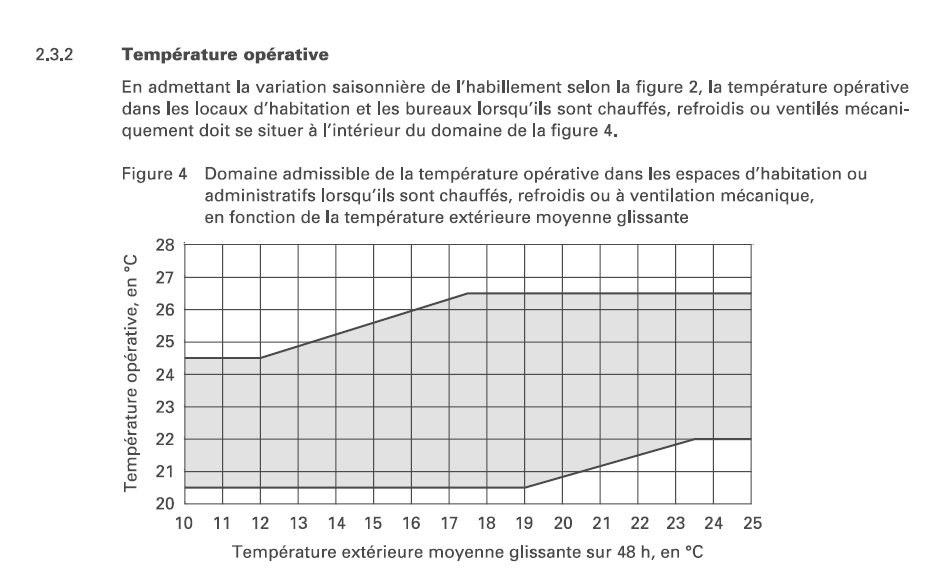
\includegraphics[height=0.75\textheight]{Images/sia_180_2014.png}
    \note[item]{Tracking the mean of the SIA 180:2014 reference temperature
    range for residental buildings. It is computed using a rolling window of
    the last 48 hours of outside temperature measurement\vspace{10pt}}
    \note[item]{Choosing this as a reference temperature provides a more
    realistic simulation scenario, as well as allowes to analyse model
    performance for a larger range of operating temperatures}
\end{frame}

% ----------------------- Implementation
\section{Implementation}

\breakingframe{
\begin{textblock*}{5cm}[0.5,0.5](0.5\textwidth,  0.5\textheight)
\Huge\textbf{\textcolor{black}{Implementation}}
\end{textblock*}
}

\begin{frame}
    \frametitle{Complete diagram}
    \centering
    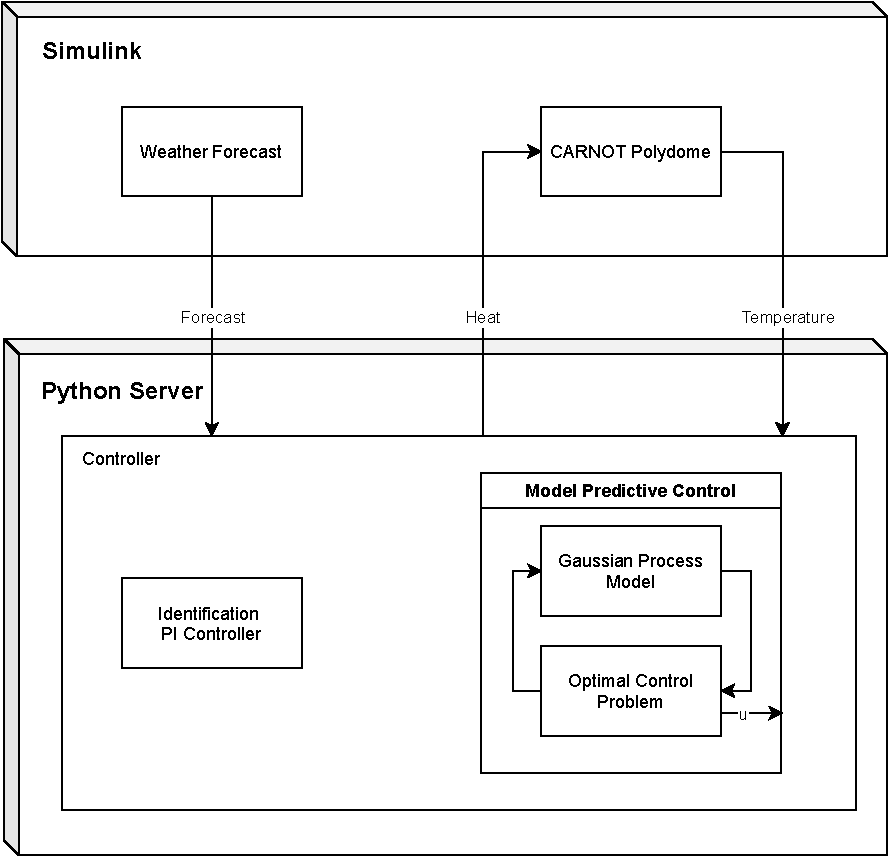
\includegraphics[height=0.75\textheight]{Images/setup_diagram.pdf}
    \note[item]{The two basic building blocks of the simulation are:
        \begin{itemize}
            \item The building model and weather prediction built in CARNOT/Simulink
            \item The control scheme implemented in Python
        \end{itemize}
    }
    \note[item]{The server starts by implementing a PI controller
    tracking the defined reference temperature until enough data has been
collected. At that point the GP model is trained and the server switches to the
MPC controller going forward}
    \note[item]{The python server is also responsible of keeping track of when
    to re-train the model in the case of adaptive schemes}
\end{frame}

\begin{frame}
    \frametitle{Simulink Diagram}
    \centering
    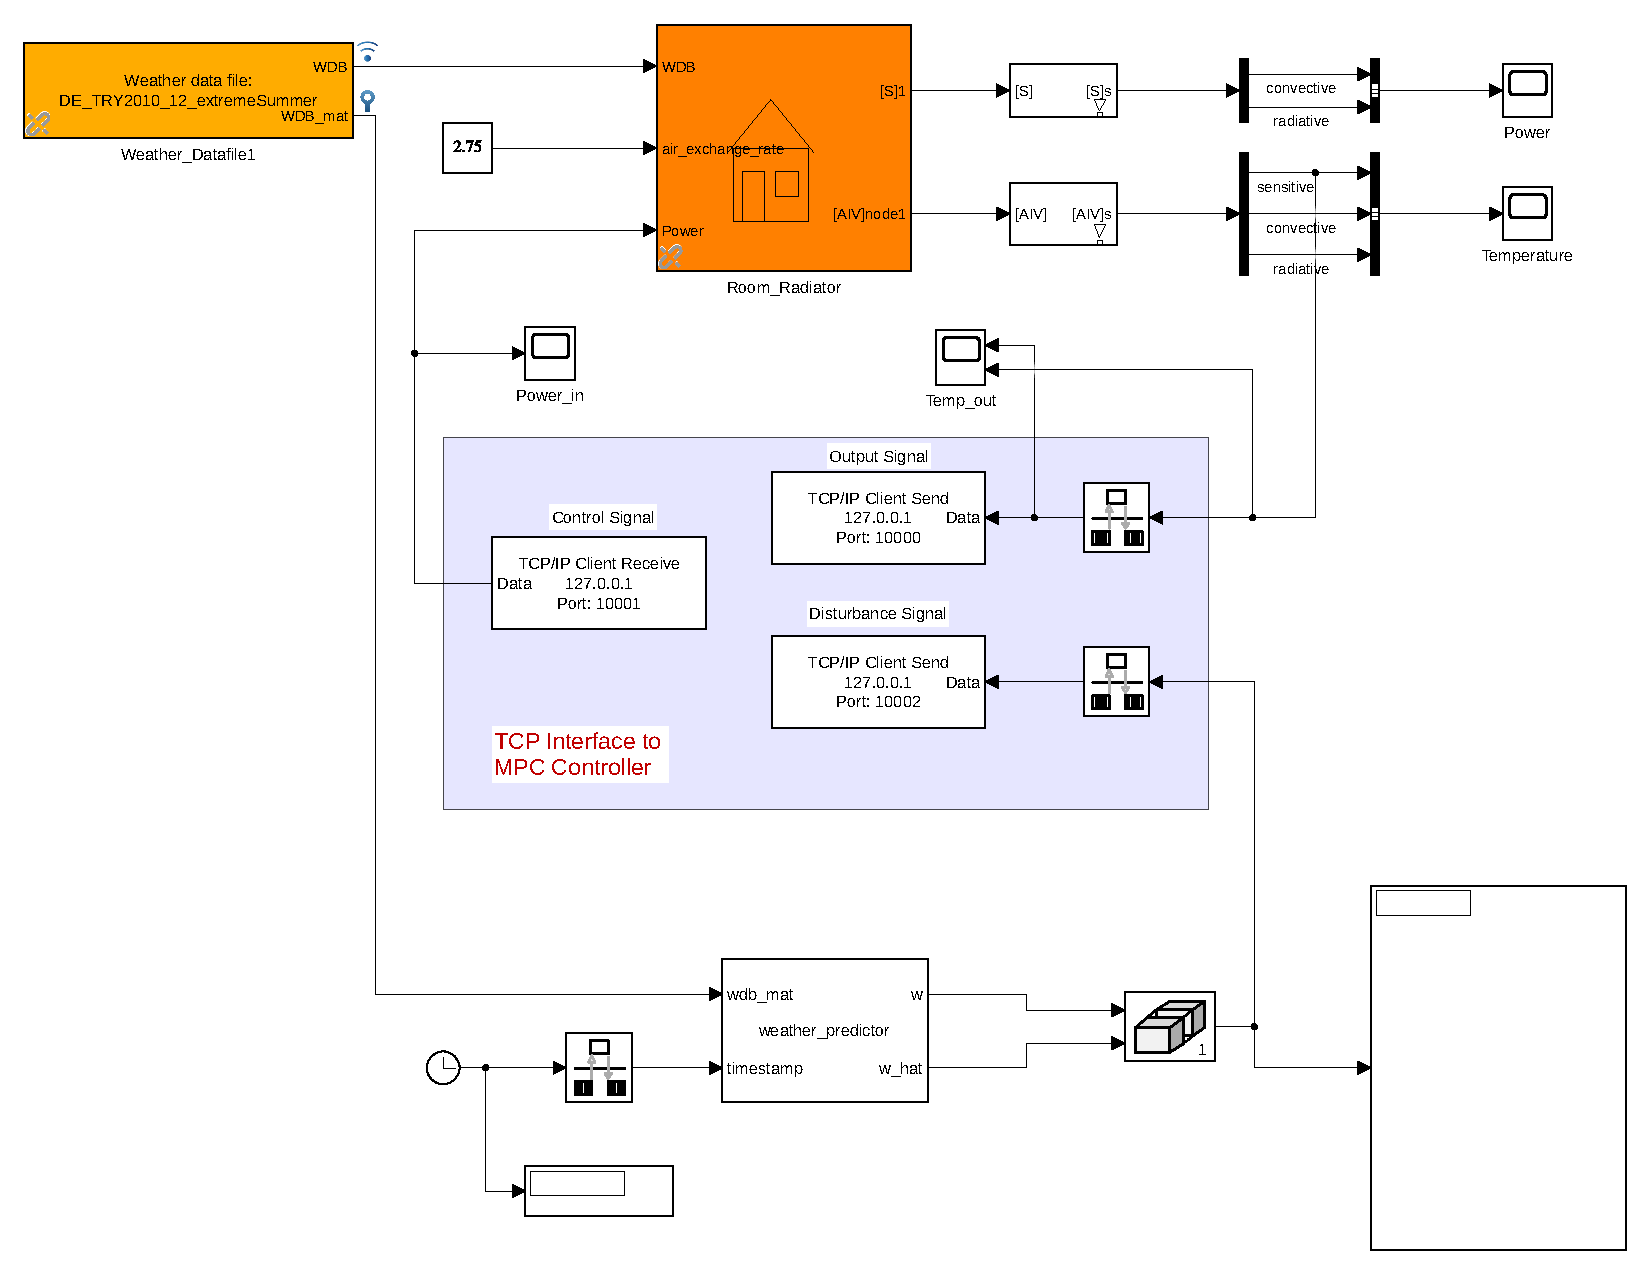
\includegraphics[height=0.75\textheight]{Images/polydome_python.pdf}
    \note[item]{The Simulink model and Python server interface through three
    independent TCP/IP sockets, each responsible for tranmission of the control
signal, measurement of the output values and the weather prediction}
\end{frame}

\begin{frame}
    \frametitle{GP implementation in Python}
    \begin{block}{GP implementation}
        \vspace{10pt}
        \begin{itemize}
            \item GP and SVGPs implemented with GPflow and Tensorflow \vspace{10pt}
            \item Optimization Problem implemented with CasADi \vspace{10pt}
        \end{itemize}
    \end{block}

    \begin{block}{Average computation time}
        \vspace{10pt}
        \begin{itemize}
            \item Classical GP optimisation step of around 1-2 s \vspace{10pt}
            \item SVGP optimisation step of around 200-300 ms \vspace{10pt}
        \end{itemize}
    \end{block}

    \note[item]{Both libraries provide very efficient implementation of all the
    required functions, leading to short computation times}
\end{frame}

% ----------------------- Simulations
\section{Full-year simulations}

\breakingframe{
\begin{textblock*}{13cm}[0.5,0.5](0.75\textwidth,  0.5\textheight)
\Huge\textbf{\textcolor{black}{Full-year simulations}}
\end{textblock*}
}

\begin{frame}
    \frametitle{GP implementations}
    \begin{block}{GP implementations for full-year simulations}
        \vspace{10pt}
        \begin{itemize}
            \item Classical GP model trained on the five days of identification
                data \vspace{10pt}
            \item SVGP model trained on five days of identification data
                \vspace{10pt}
            \item SVGP model trained on one day of identification data
                \vspace{10pt}
            \item SVGP model trained on a rolling window of five days of
                closed-loop operation data \vspace{10pt}
        \end{itemize}
    \end{block}
\end{frame}

\begin{frame}
    \frametitle{Classical GP full year simulation}
    \centering
    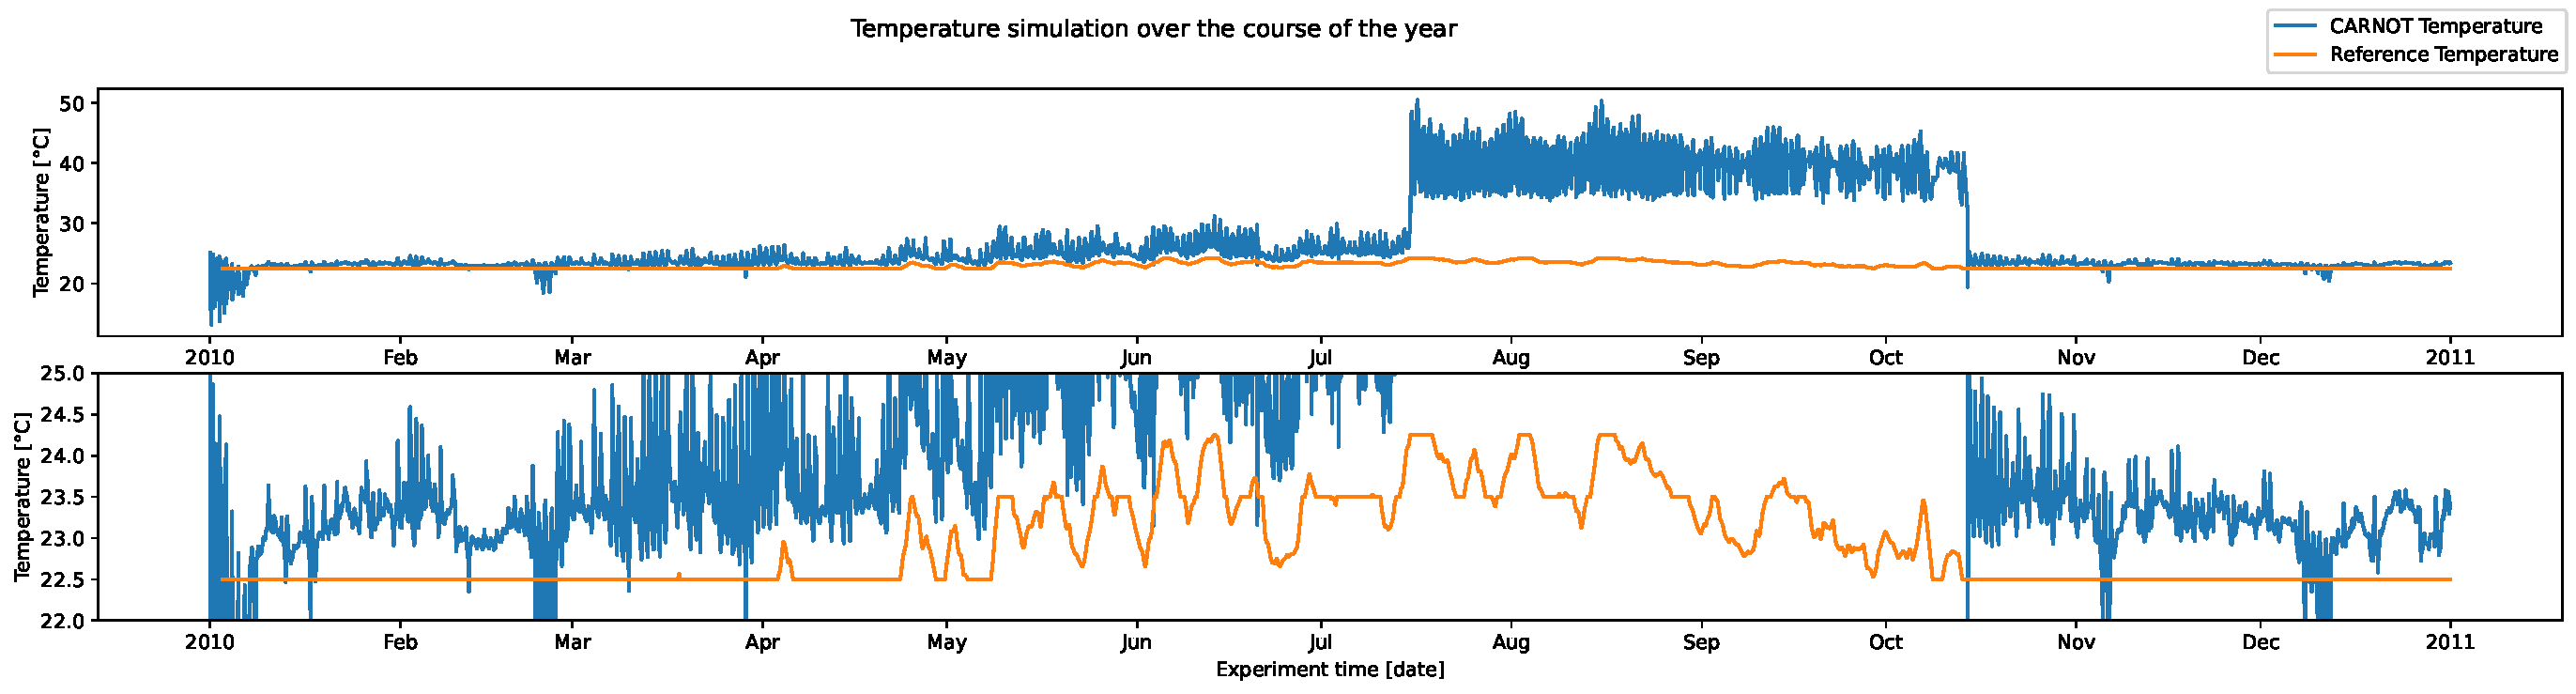
\includegraphics[width=0.85\textwidth]{Plots/4_GP_480pts_12_averageYear_fullyear.pdf}
    \note[item]{From the first result it can be seen that the classical GP does
    not perform well. It has a very large offset from the start of the
simulation and becomes completely unstable in late summer}
\end{frame}

\begin{frame}
    \frametitle{Absolute Error graph}
    \centering
    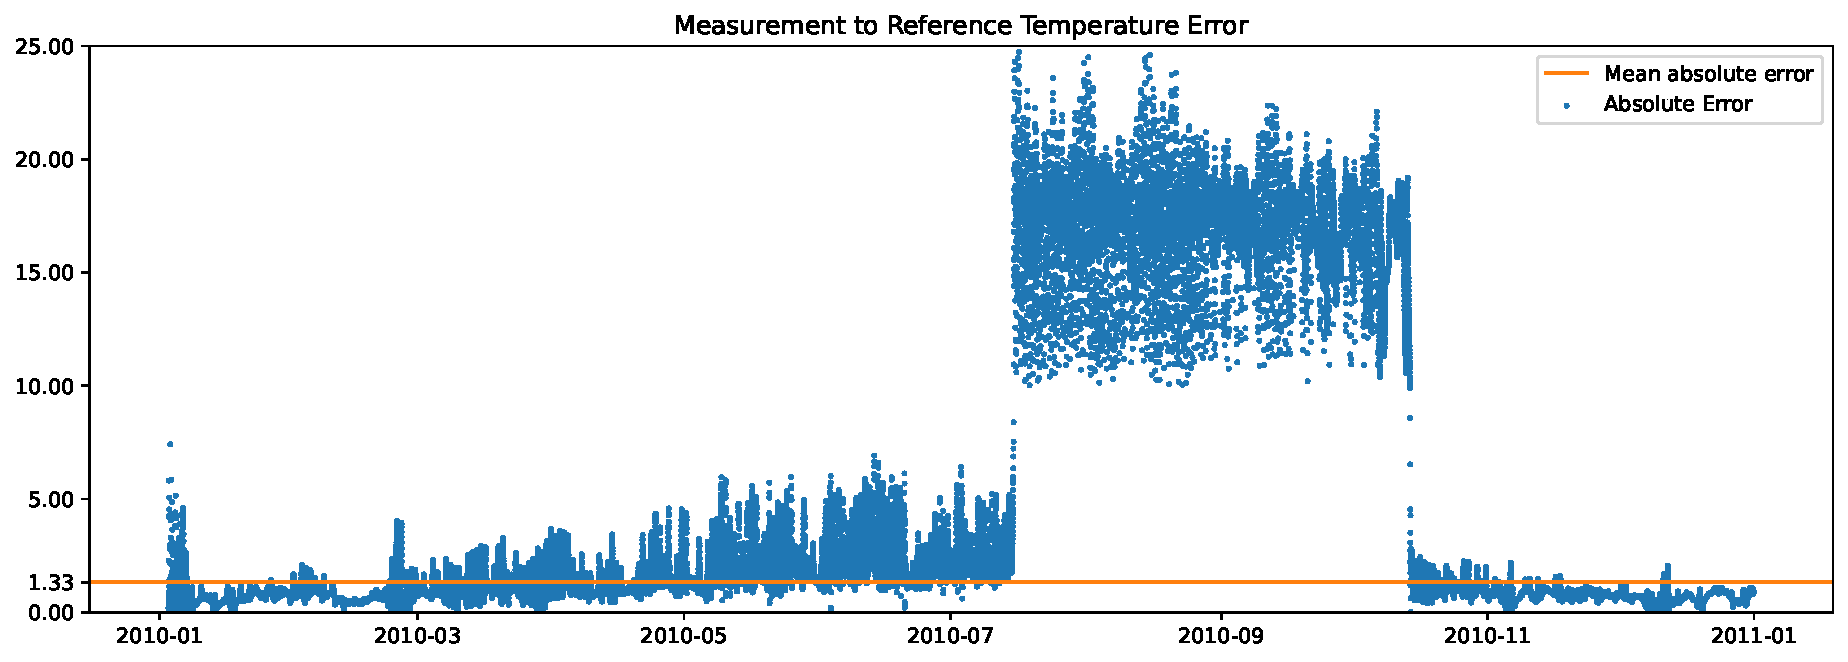
\includegraphics[width=\textwidth]{Plots/4_GP_480pts_12_averageYear_abserr.pdf}
    \note[item]{A more quantitative analysis shows a maximum absolute error of
    aroun 25 degrees C, with the mean over the whole year being 1.33 degrees C}
\end{frame}

\begin{frame}
    \frametitle{GP model performance}
    \centering
    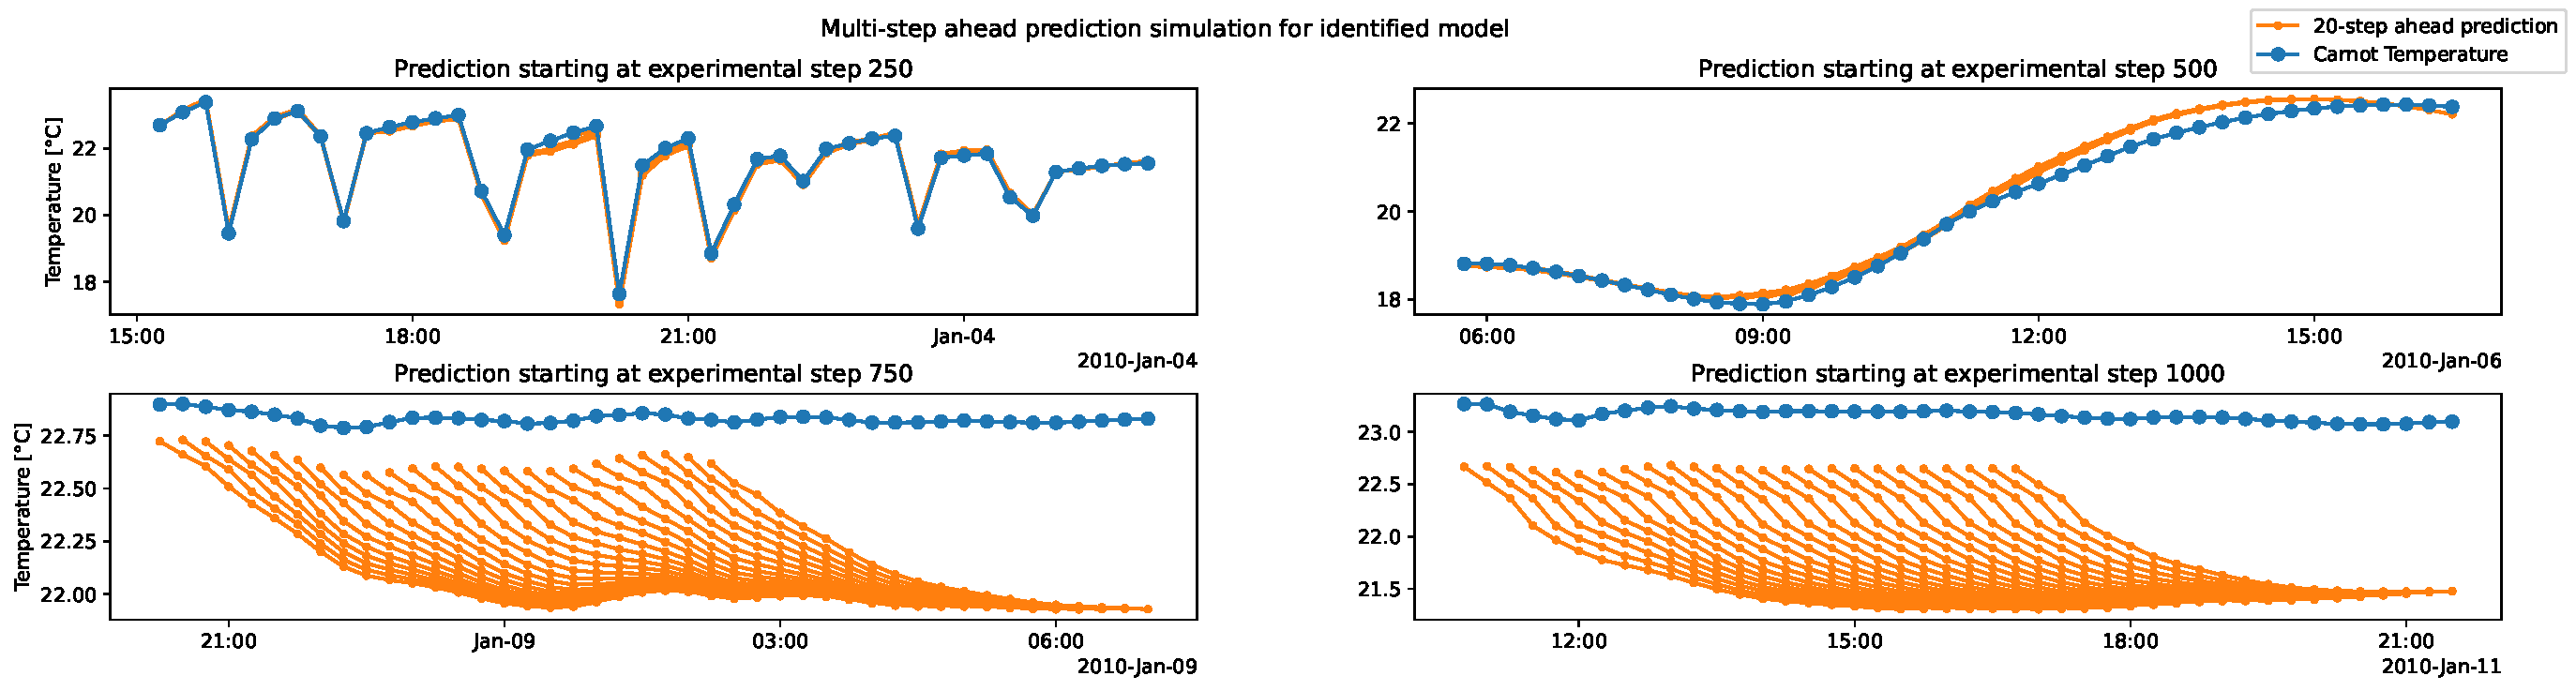
\includegraphics[width=\textwidth]{Plots/4_GP_480pts_12_averageYear_first_model_performance.pdf}
    \note[item]{Very good multistep ahead performance in the training region,
    the model correctly reproduces learned data}
    \note[item]{At step 500 the model is able to correctly predict the heating
    of the building to the 22.5 degrees C reference temperature}
    \note[item]{Already at step 750, on the ninth day of the simulation, the
    model is unable to properly predict building behaviour and settles on a
    steady-state prediction error of ~0.75 degrees C.}
    \note[item]{Even worse performance at experimental step 1000, where the
    steady-state error is around 1.5 degrees C}
\end{frame}

\begin{frame}
    \frametitle{Disturbance signal}
    \centering
    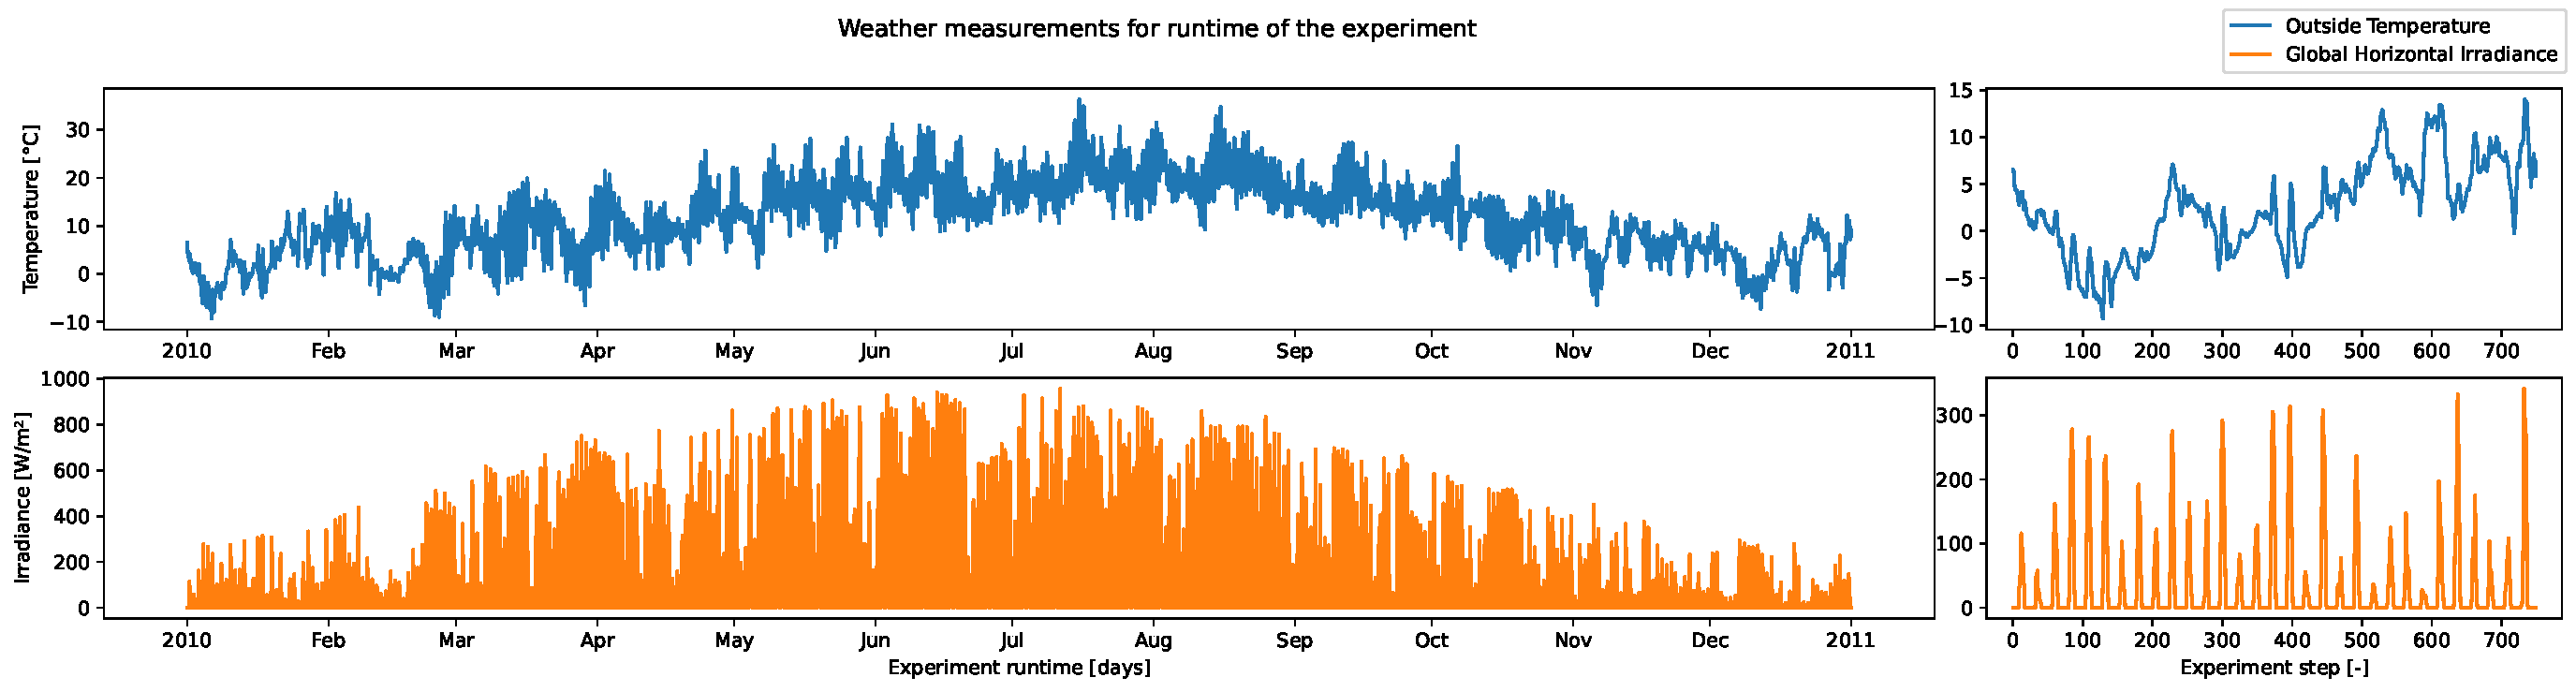
\includegraphics[width=\textwidth]{Plots/Exogenous_inputs_fullyear.pdf}
    \note[item]{The weather patterns are representative of Switzerland, with
    generally mild winters and temperate summer, but the weather does not remain
constant throughout the year\vspace{10pt}}
    \note[item]{Both disturbance inputs, the outside temperature and the global
    irradiation are outside the learning dataset region already around the 500
point mark}
    \note[item]{This forces the GP model to work in an extrapolated region of
    the state space, which it did not see during training. In this situation the
GP model does not perform well\vspace{10pt}}
    \note[item]{The window of values for the two disturbance signals keeps
    expanding until mid summer, after which both values start decreasing again.
This is useful for training the SVGP models.}
\end{frame}


\begin{frame}
    \frametitle{SVGP full year simulation}
    \centering
    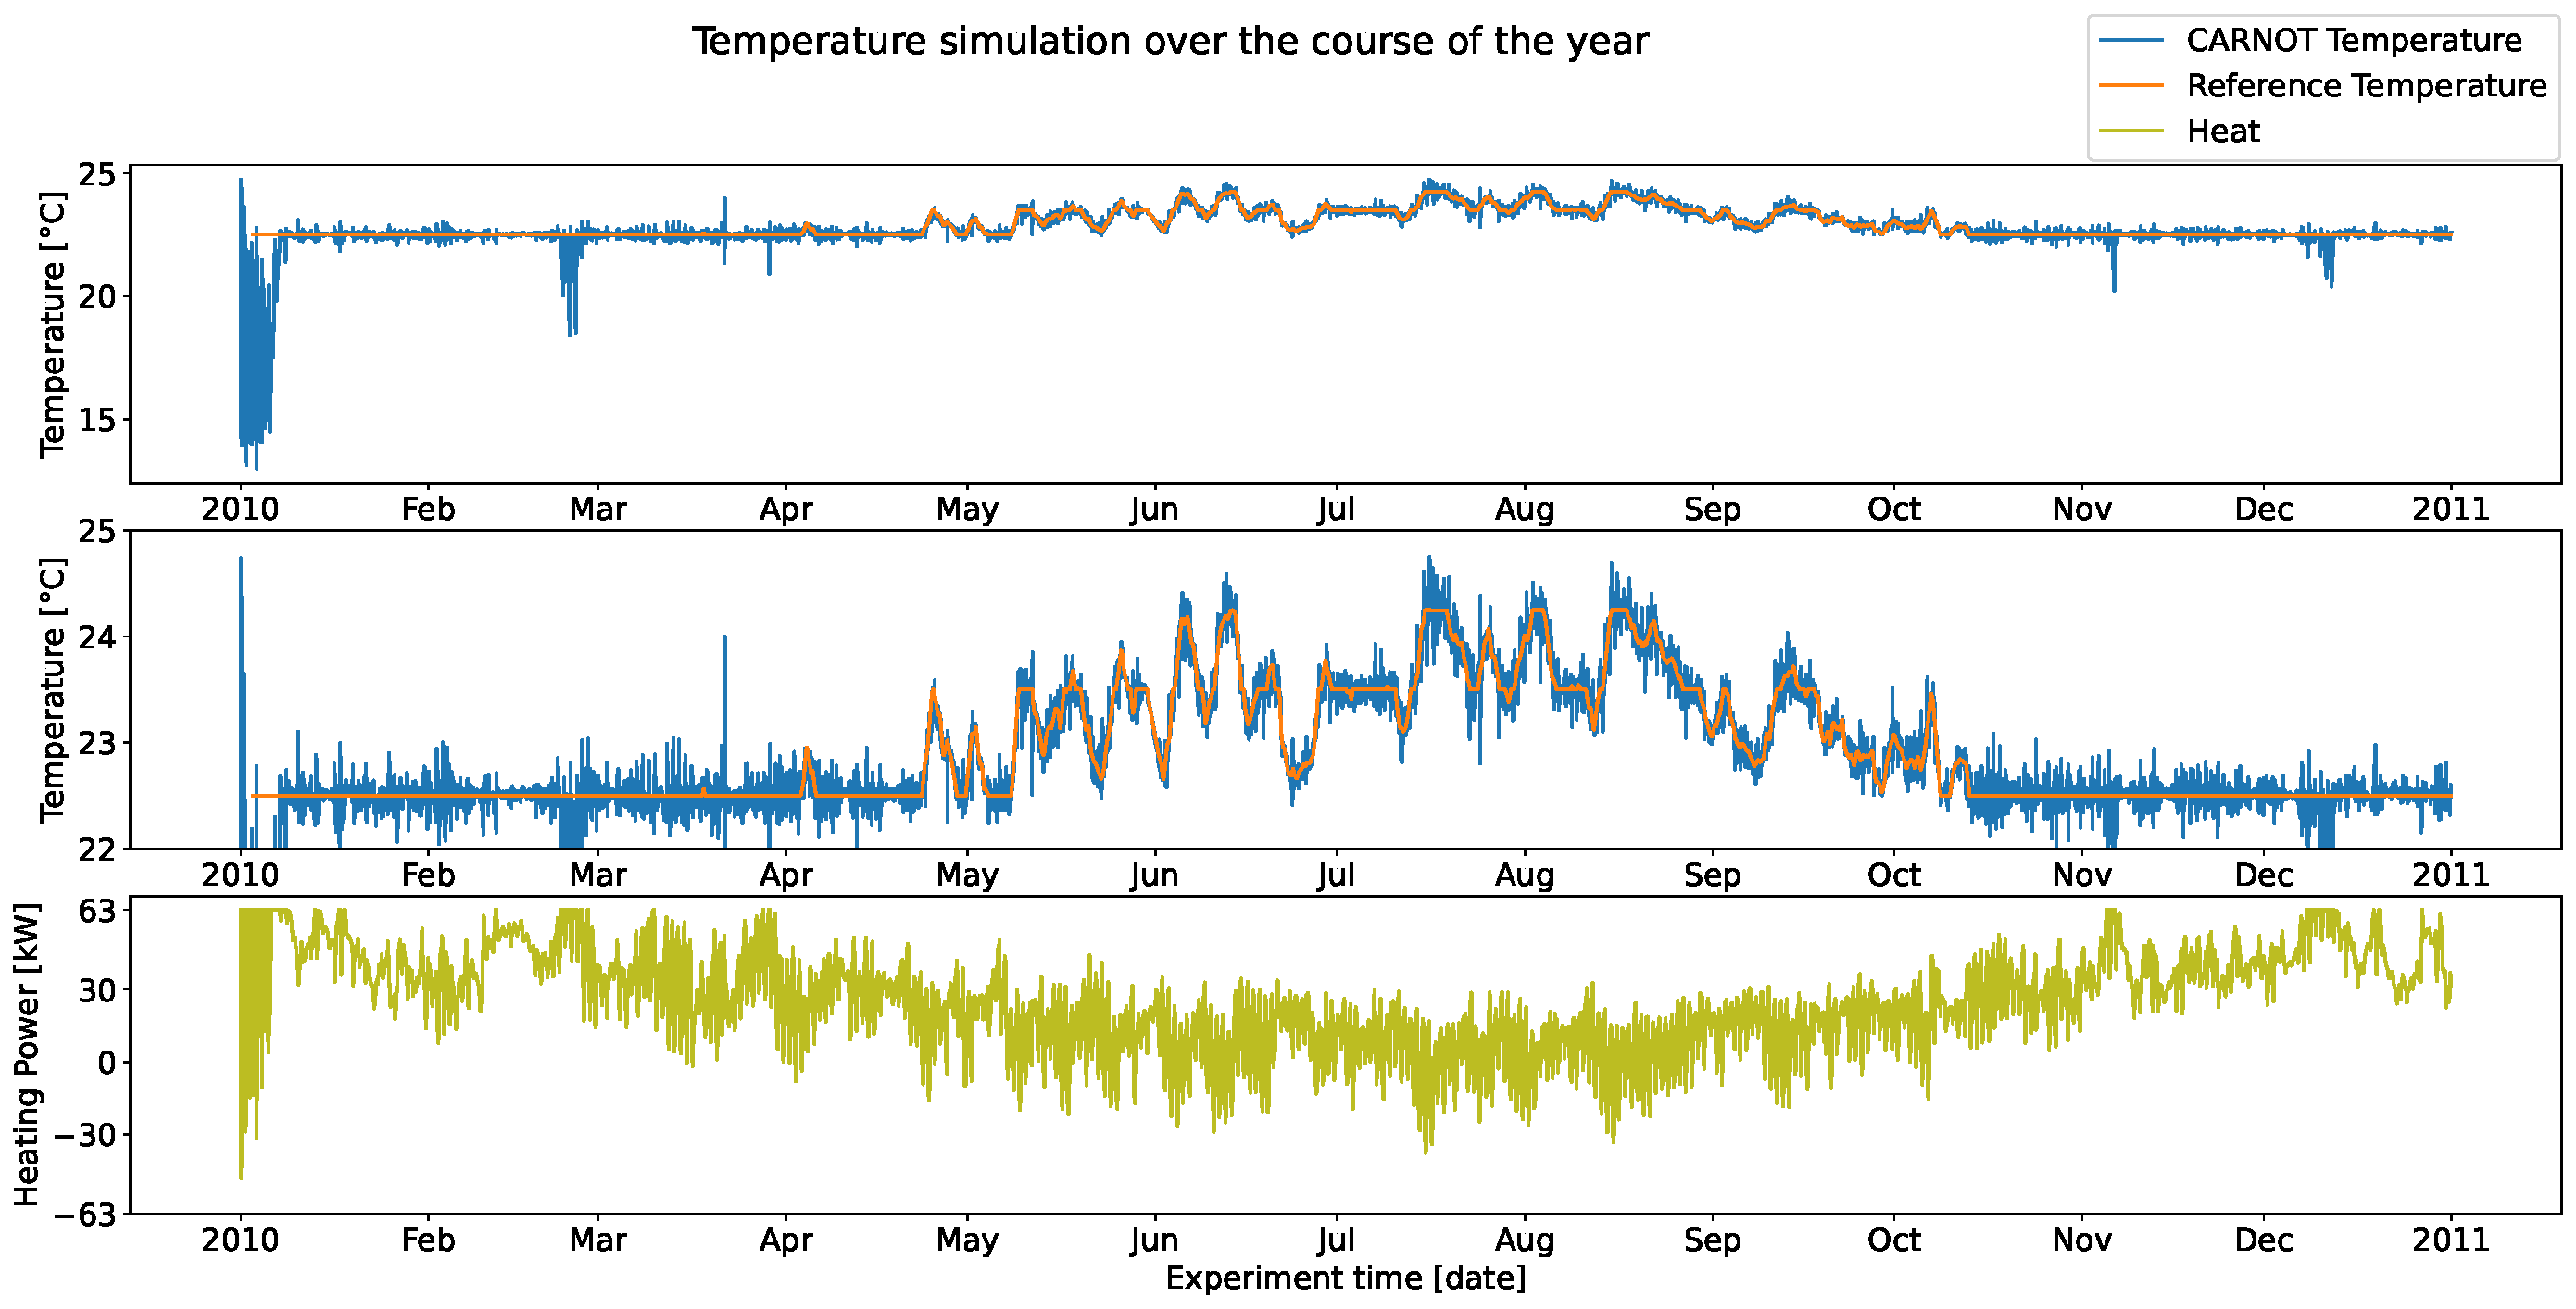
\includegraphics[width=0.85\textwidth]{Plots/1_SVGP_480pts_inf_window_12_averageYear_fullyear.pdf}
    \note[item]{Much better performance than the classical GP system}
    \note[item]{The only large deviations from the reference temperatures are in
    the winter, when the HVAC heat supply is at its limit.}
    \note[item]{The constant model updates mean that the model does not have to
    extrapolate as far in the unknown regions before new data is added}
\end{frame}

\begin{frame}
    \frametitle{Absolute Error graph}
    \centering
    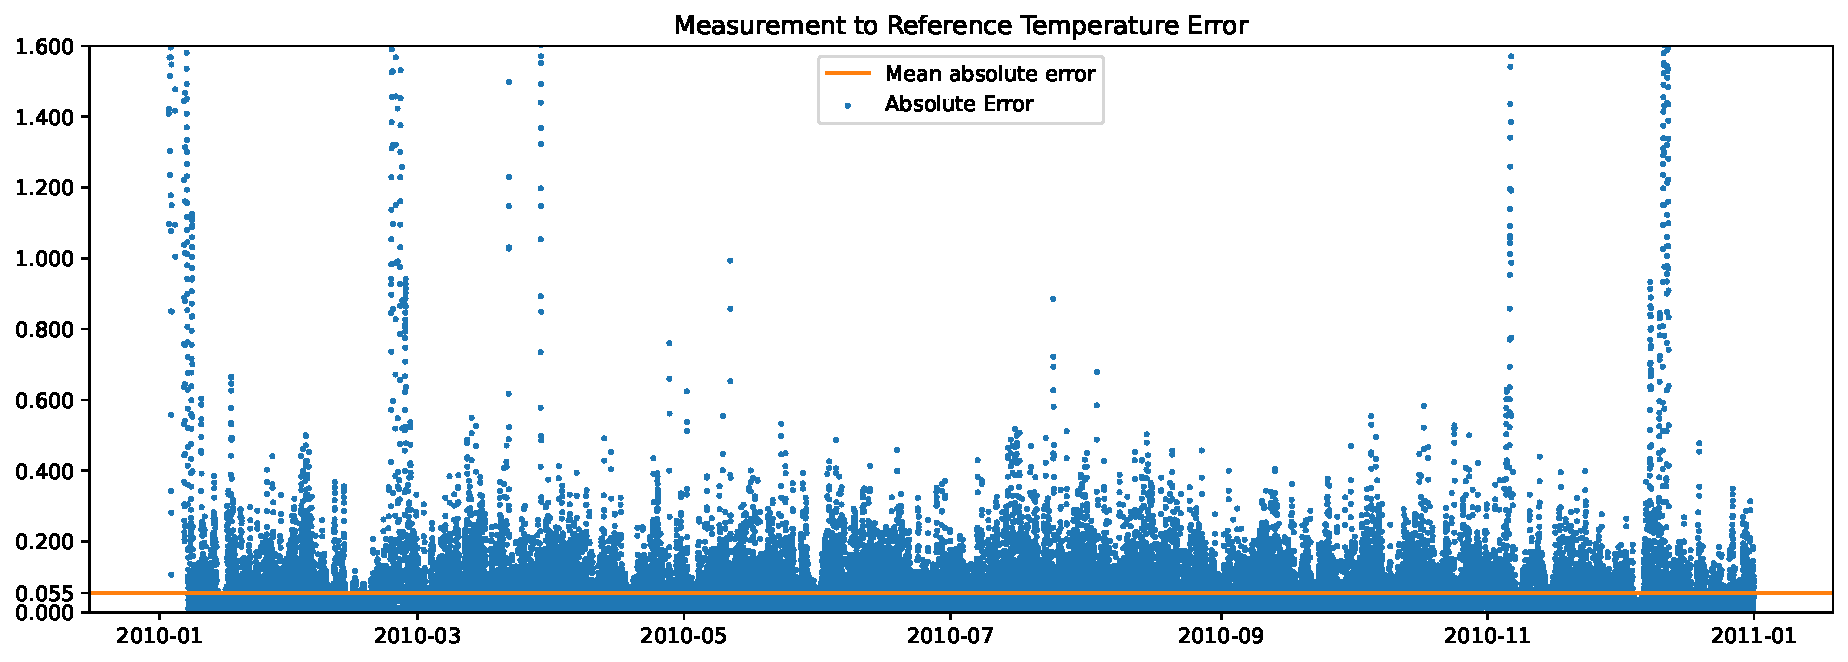
\includegraphics[width=\textwidth]{Plots/1_SVGP_480pts_inf_window_12_averageYear_abserr.pdf}
    \note[item]{Quantitavely a much better result, with a maximum absolute error of
    around 1.6 degrees, except the cold days limited by the HVAC power}
    \note[item]{An average absolute error over the whole year of ~0.055 degrees
    C}
\end{frame}

\begin{frame}
    \frametitle{SVGP model performance}
    \centering
    \movie[width=\textwidth]{
        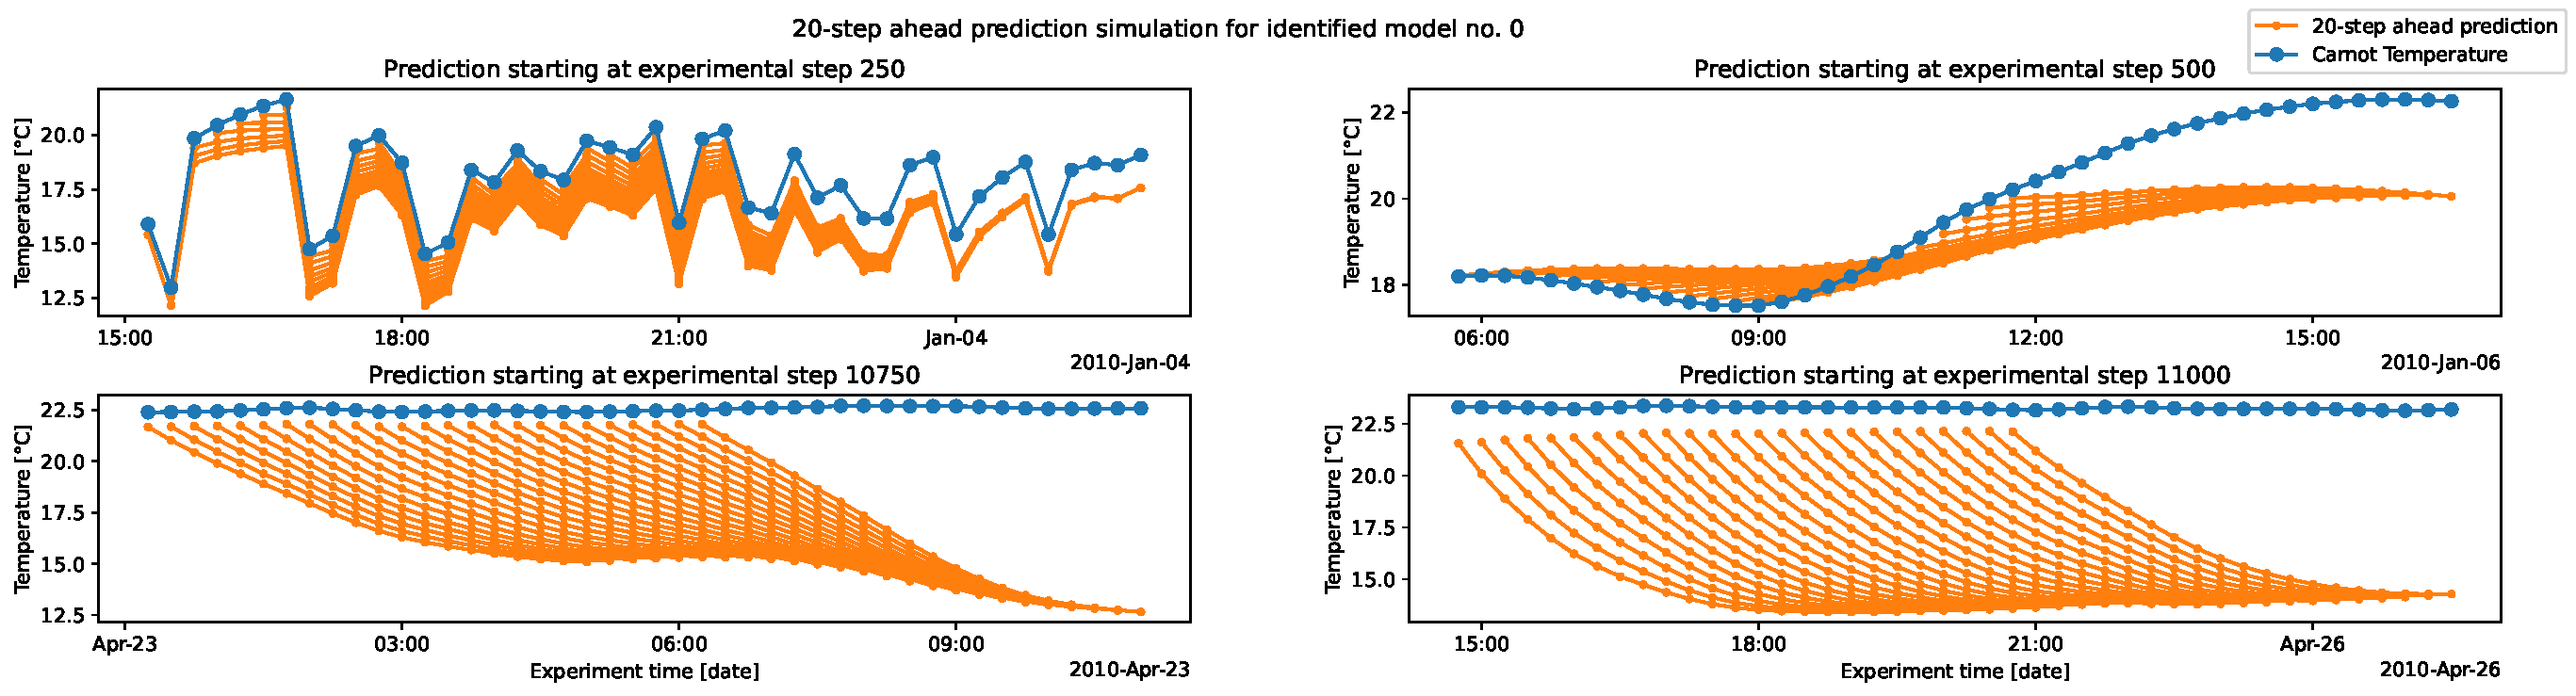
\includegraphics[width=\textwidth]{Plots/1_SVGP_480pts_inf_window_12_averageYear_model_0_performance.pdf}}
        {Plots/SVGP_perf_animation.mkv}
    \note[item]{Play the simulation movie}
    \note[item]{Overall two large families of models. During the first part of
    the year, as the range of the weather data gets expanded the predictions get
progressively better. For the second part of the year the range of the data does
not get expanded anymore and the performance of the model becomes noticeably
better}
    \note[item]{The multistep prediction performance of the SVGP over the
    training region (ie. at 250 steps) starts much worse than that of the
equivalent GP. This could be a sign that more inducing variables are necessary
to properly reproduce the training data}
\end{frame}

\begin{frame}
    \frametitle{SVGP one day starting data}
    \centering
    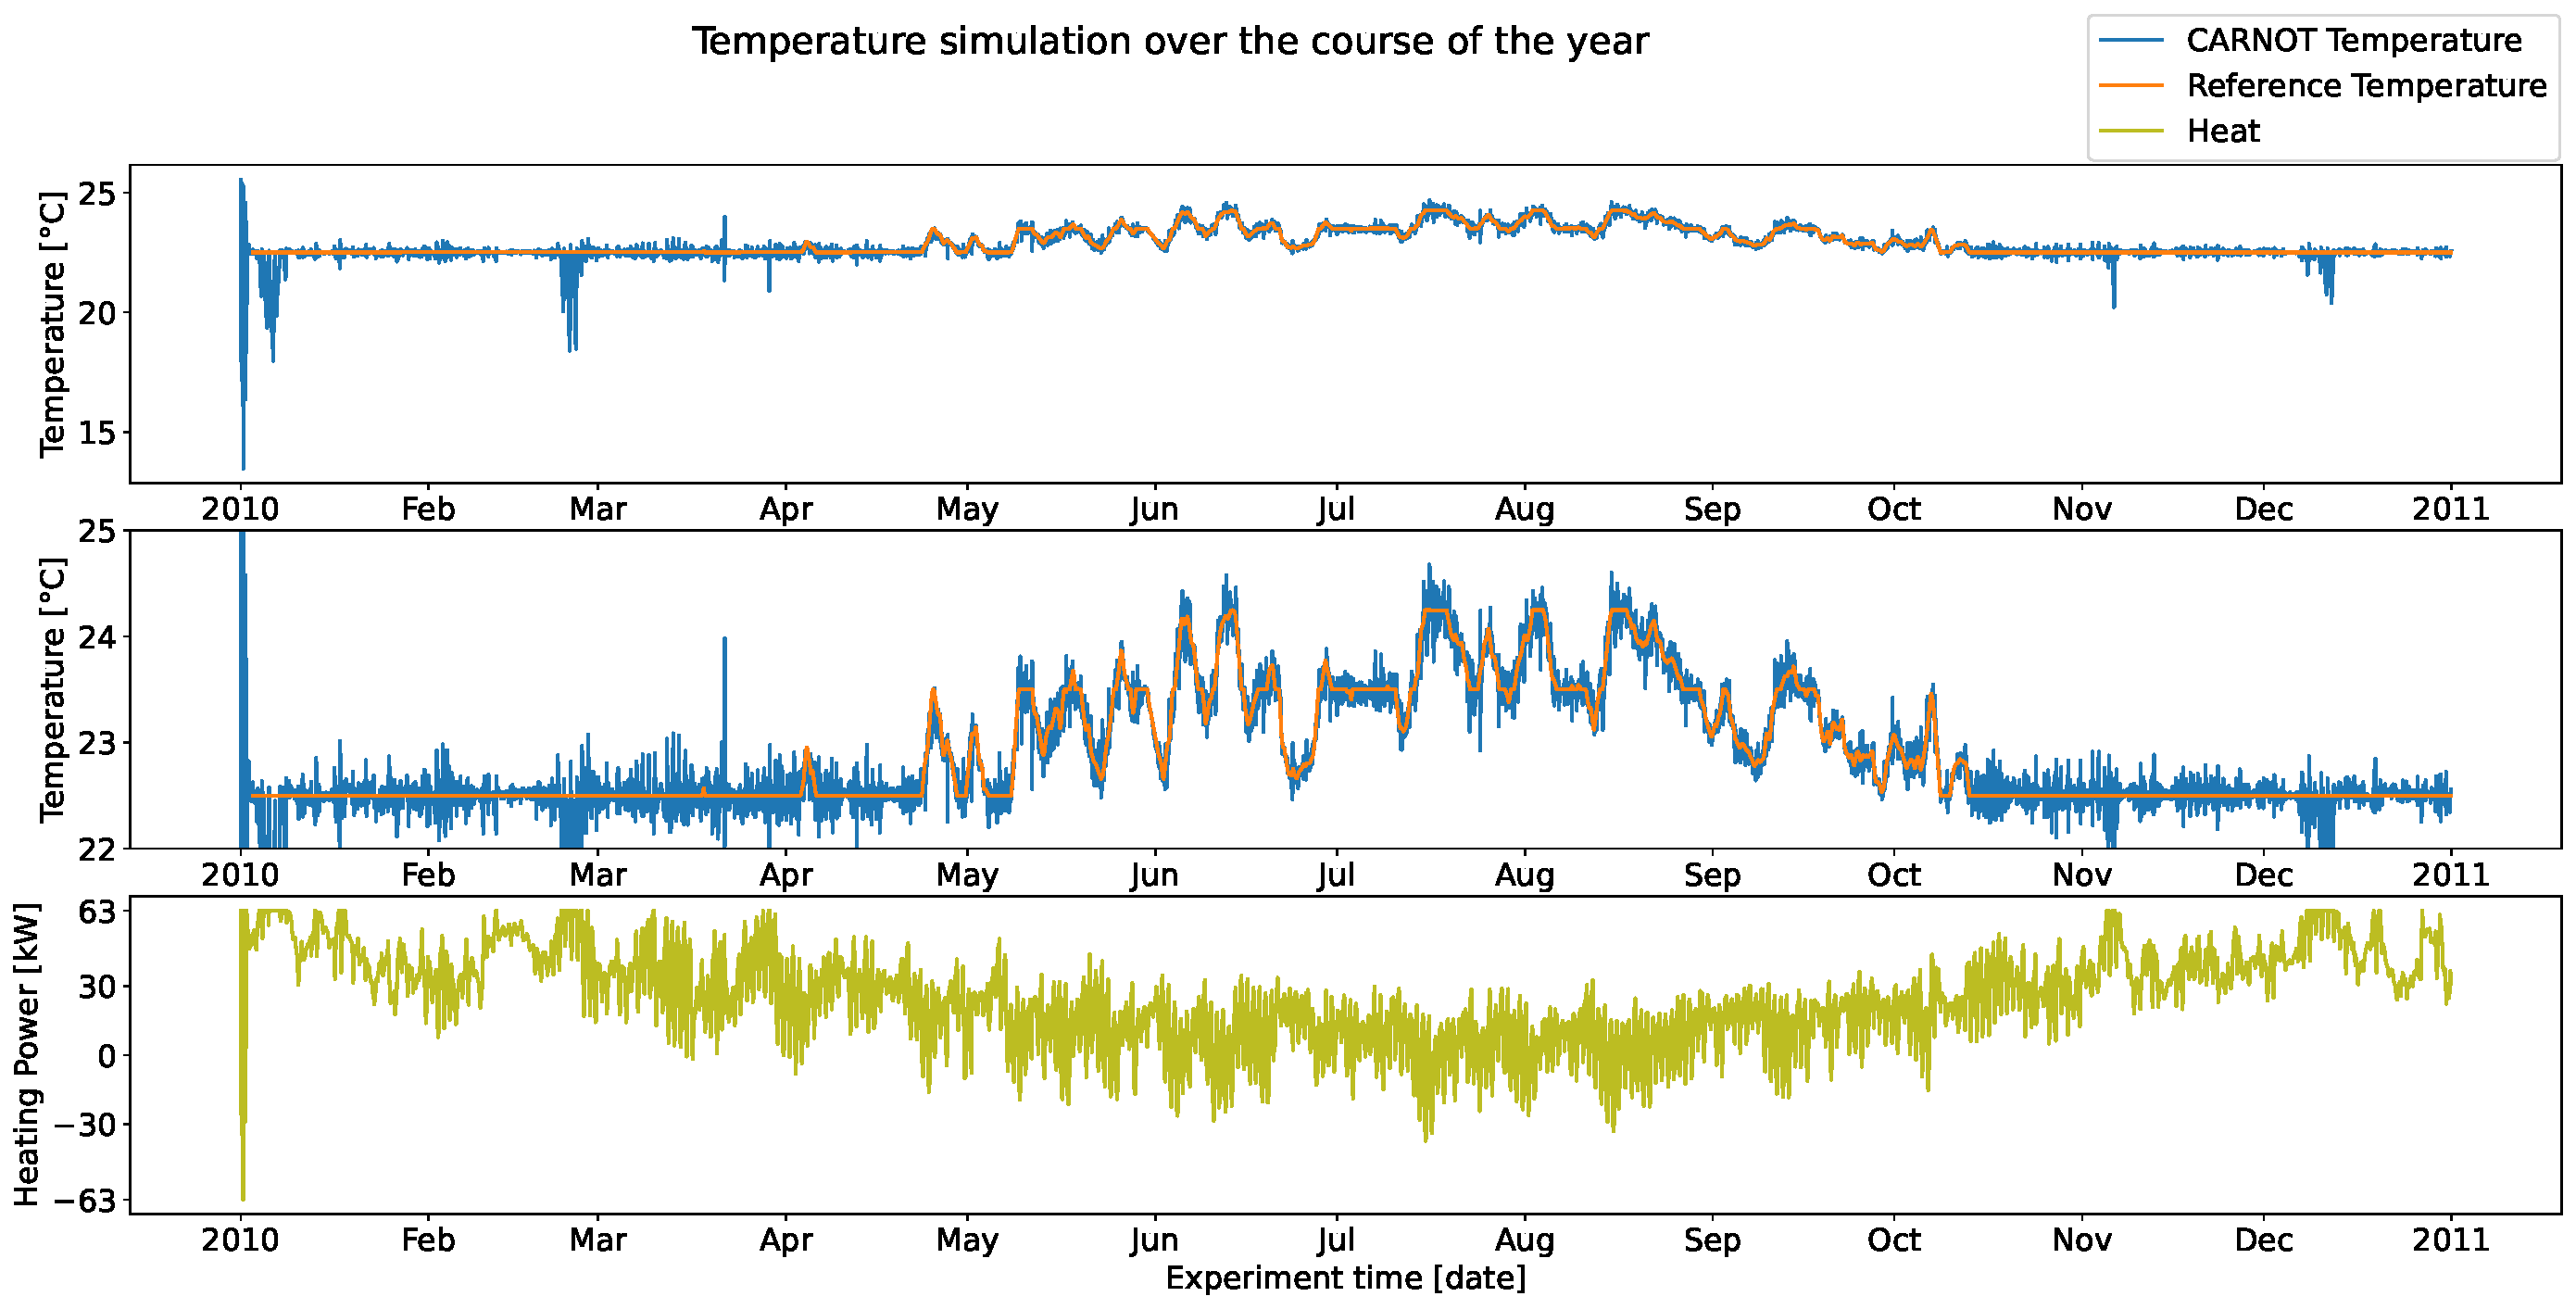
\includegraphics[width=0.85\textwidth]{Plots/6_SVGP_96pts_inf_window_12_averageYear_fullyear.pdf}
    \note[item]{Performance very comparable to that of five days initial model}
    \note[item]{This hints at the fact that SVGP models can be deployed using
    much less initial training data than traditional GP models, and are still
capable of good performance from learned behaviour}
\end{frame}

\begin{frame}
    \frametitle{SVGP five day rolling window}
    \centering
    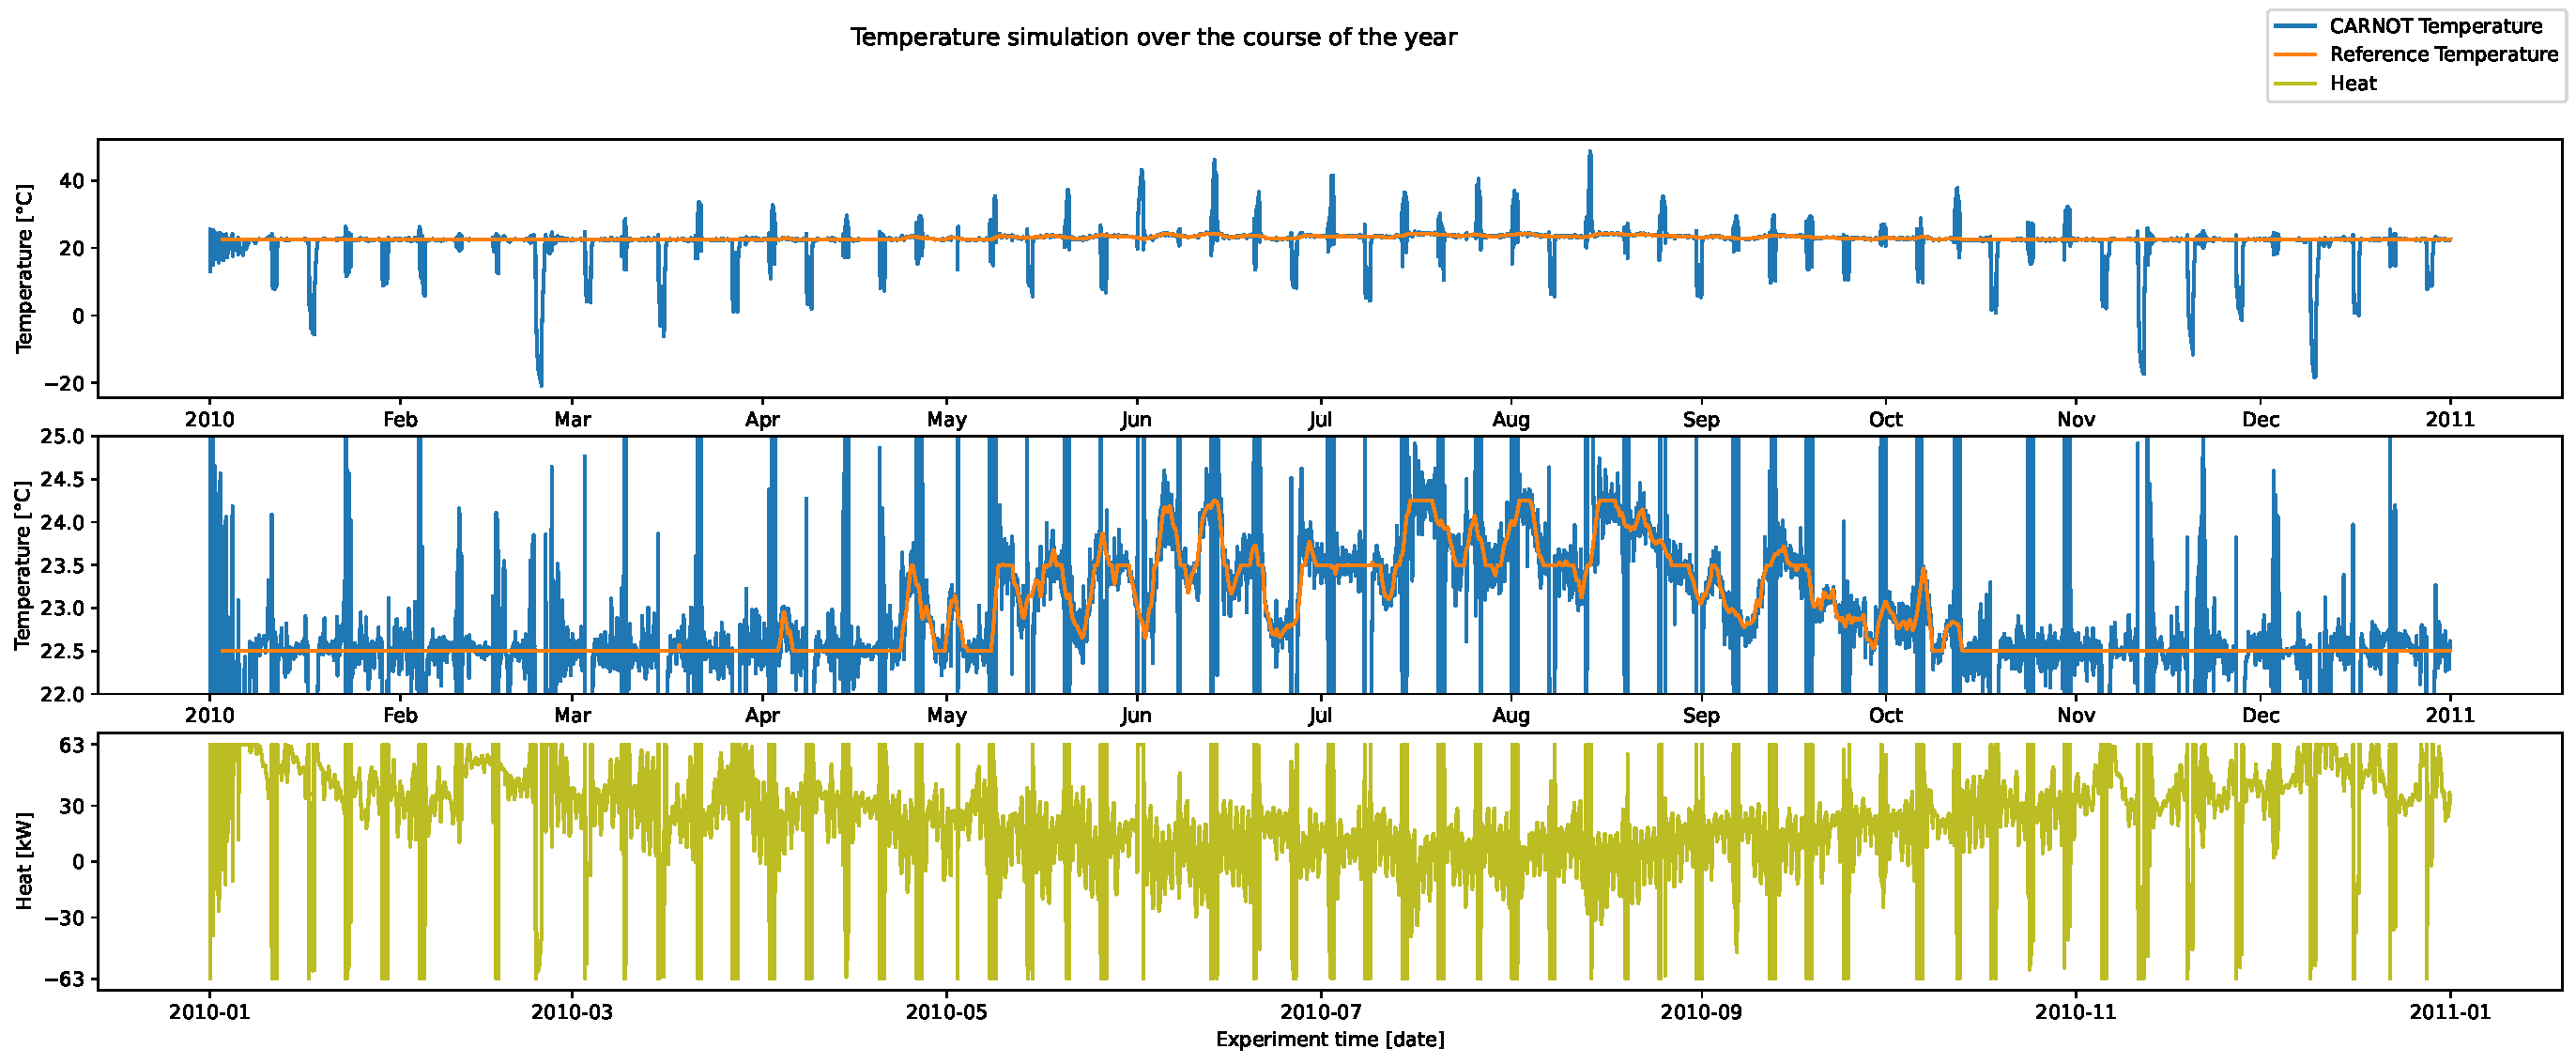
\includegraphics[width=0.85\textwidth]{Plots/5_SVGP_480pts_480pts_window_12_averageYear_fullyear.pdf}
    \note[item]{Five days worth of initial training data. After five days of
    operation, the rolling window of training data does not contain any initial
    identification anymore, only closed loop operation data. This information turns
    out to be insufficient for learning the plant behaviour and the controller
    becomes unstable.}
    \note[item]{The additional excitation of the model in turn provides enough
    information for the next model to properly capture its behaviour, turning
    the controller stable again until the data containing the excitations is too old
    again to include in the training set.}
\end{frame}

\begin{frame}
    \frametitle{SVGP linear kernel}
    \centering
    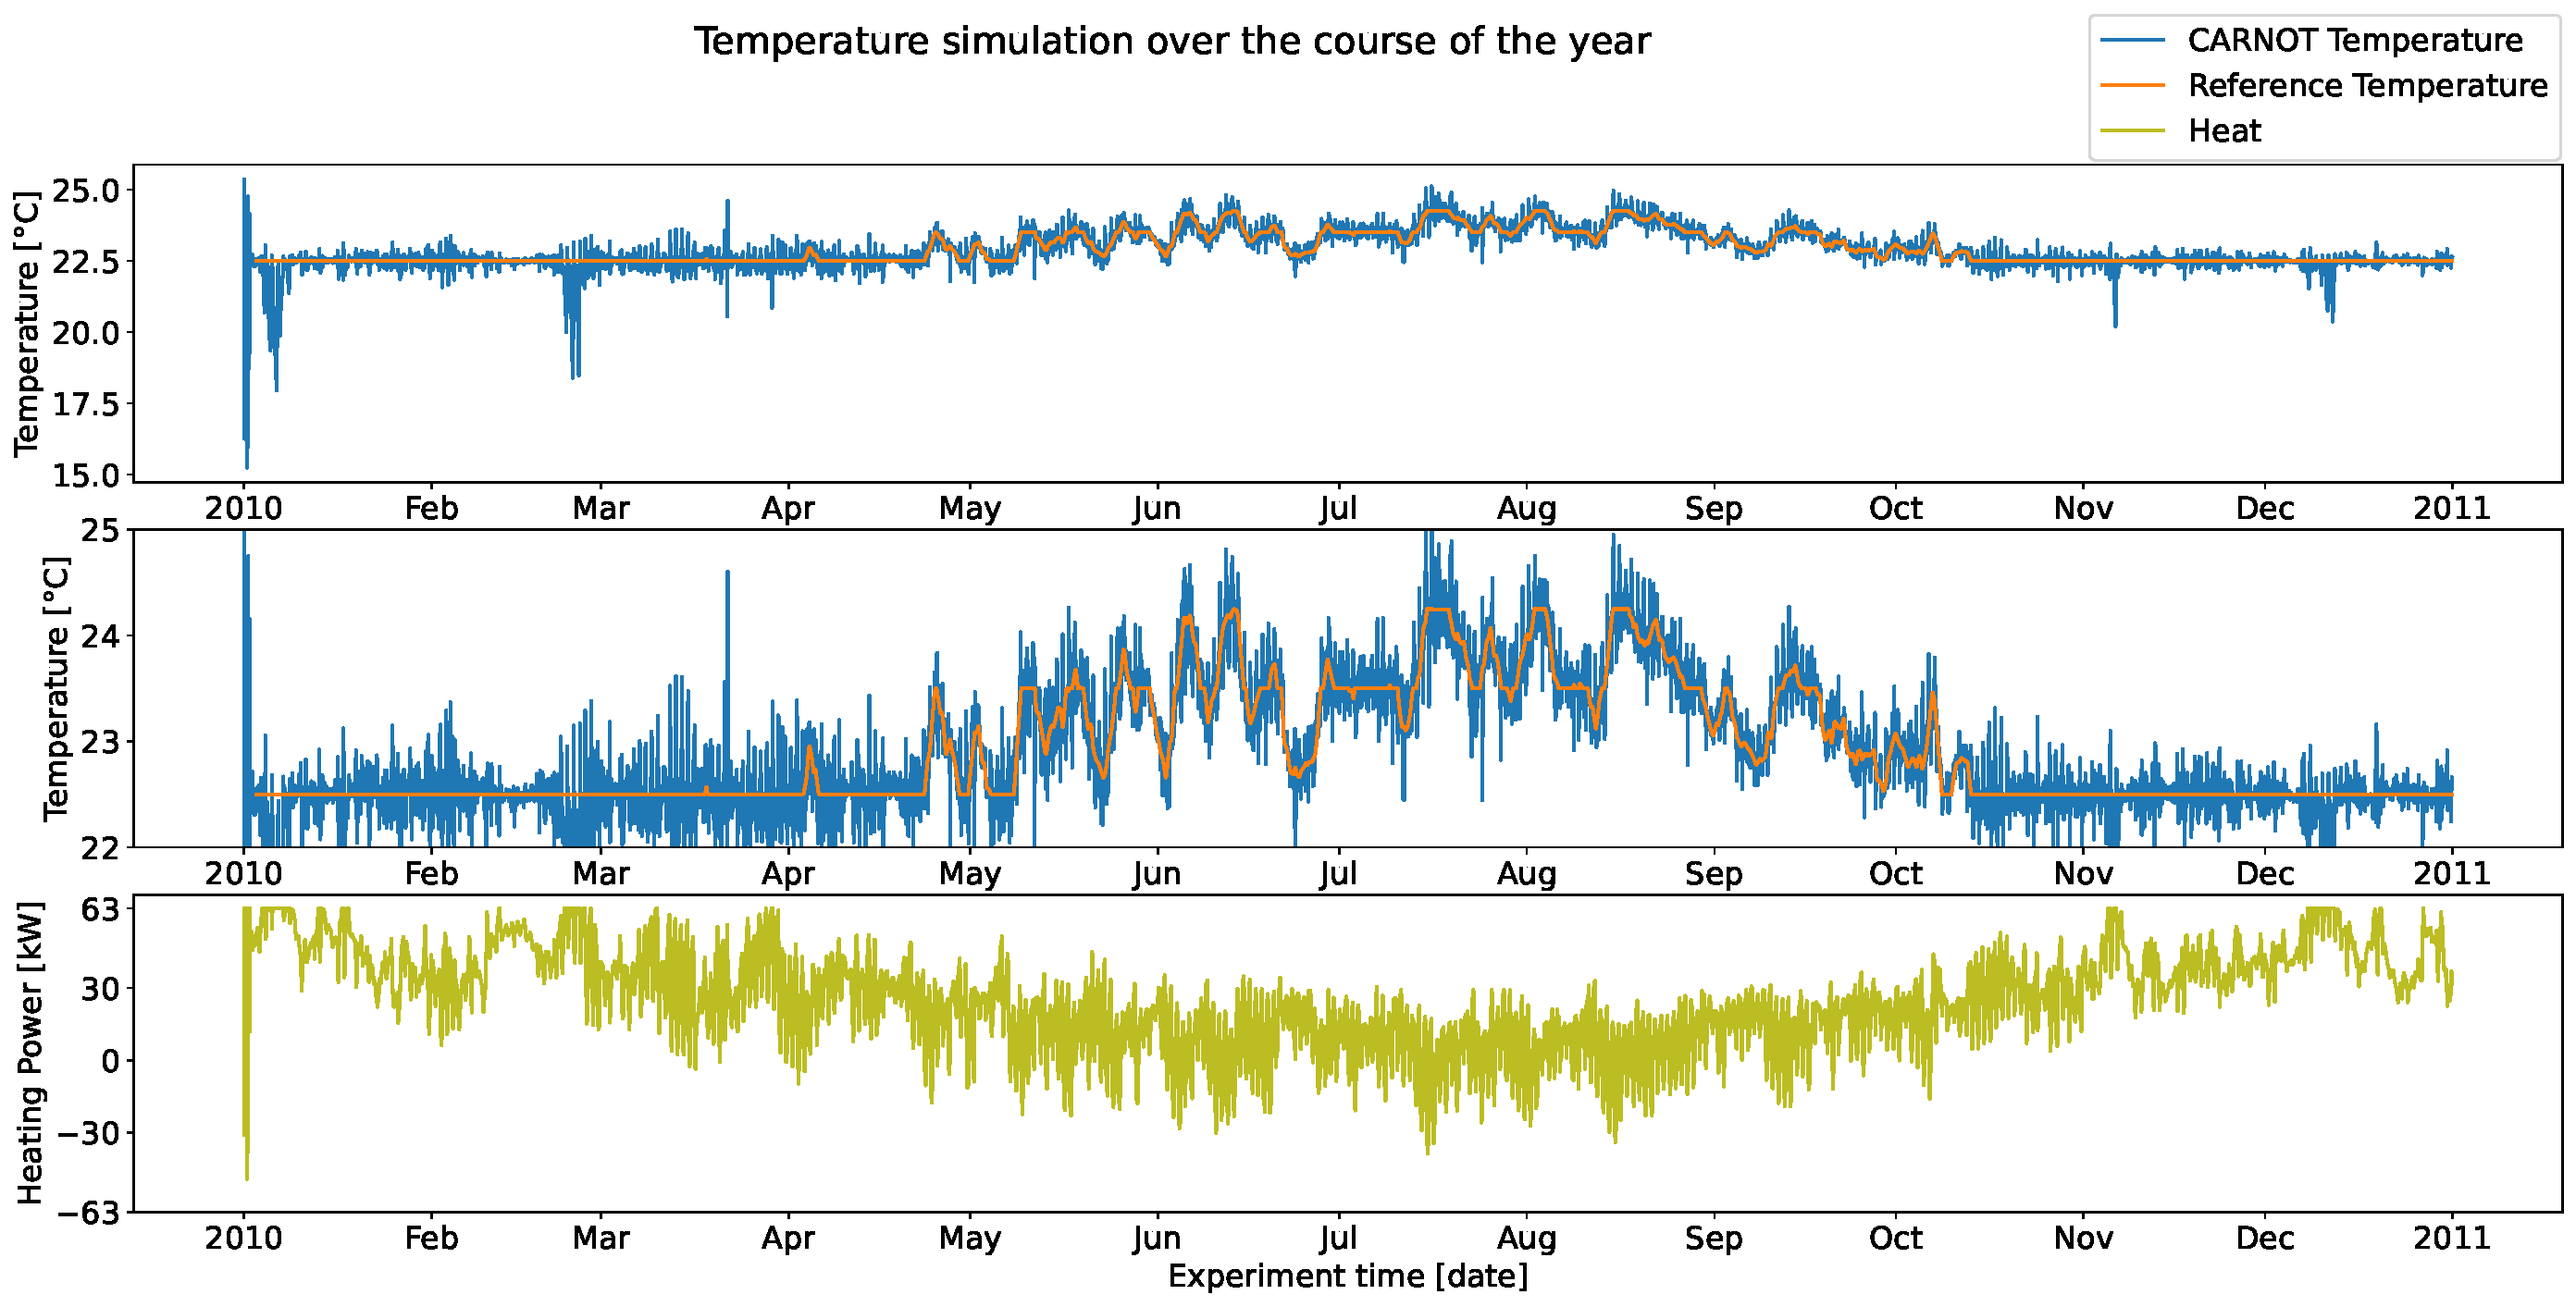
\includegraphics[width=0.85\textwidth]{Plots/10_SVGP_480pts_inf_window_12_averageYear_LinearKernel_fullyear.pdf}
    \note[item]{This model is still stable and able to roughly follow the
    reference temperature. It has, however poorer performance than the main
model, trained using a Squared Exponential Kernel. This means that the Linear
Kernel is too simplistic for even this situation.}
\end{frame}

% ----------------------- Future work
\section{Future Work}

\breakingframe{
\begin{textblock*}{10cm}[0.5,0.5](0.75\textwidth,  0.5\textheight)
\Huge\textbf{\textcolor{black}{Future work}}
\end{textblock*}
\note[item]{Several situations have not been thoroughly addressed in this
work and could be further investigated, as well as multiple directions for
direct continuation of this project are possible}
}

\begin{frame}
    \frametitle{Future work}
    \begin{itemize}
        \item A more varied initial dataset for the classical Gaussian Process
            \vspace{10pt} \pause
        \item Smart update of a fixed-size data dictionary according to
            information gain \vspace{10pt} \pause
        \item Sparse GP wihout the use of variational inference \vspace{10pt}
            \pause

        \item The size of the inducing variables set can be further optimized
            \vspace{10pt} \pause

        \item More specialized kernel functions can be very beneficial in the
            case of SVGP models
    \end{itemize}

    \note[item]{Varied initial dataset can be more representative of the
    plant operating region over long timespans, improving overall model quality
    \vspace{10pt}}

    \note[item]{Keeping a dictionary will inevitably aleviate some of the
    downsides of using classical Gaussian Processes, at the cost of much more
    expensive computations for model update
    \vspace{10pt}}

    \note[item]{Not using variational inference in the form of the Evidence
    Lower Bound can provide a model that better explains the training data, at
    the expense of longer training time}

    \note[item]{More complex are refined kernel functions can greatly improve
    behaviour in the case of SVGP models as they are less capable of capturing
    plant dynamics as the classical GP counterpart, given the same training dataset}

\end{frame}


% -----------------------References
% Thank you slide should be here
\breakingframe{
\begin{textblock*}{10cm}(3.2cm,4cm)
\Huge\textbf{\textcolor{black}{Thank you for your attention}}
\end{textblock*}
}
\breakingframe{
\begin{textblock*}{10cm}(3.2cm,4cm)
\Huge\textbf{\textcolor{black}{Questions}}
\end{textblock*}
}
% -----------------------References
\section{Bibliography}
% \begin{frame}[allowframebreaks]{\\References}\vspace{4pt}
\begin{frame}{References}\vspace{4pt}
\tiny{\printbibliography}
\end{frame}
\normalsize

\end{document}
